\documentclass[12pt,a4paper]{article}
\usepackage[a4paper, margin=0.8in, headheight=14pt]{geometry}
\usepackage{fontspec}
\usepackage{unicode-math}
\setmainfont{TeX Gyre Pagella}
\setmonofont[Scale=0.88]{TeX Gyre Cursor}
\setmathfont{Latin Modern Math}
\usepackage{xcolor}
\usepackage{colortbl}
\usepackage{titlesec}
\usepackage{enumitem}
\usepackage{tabularx}
\usepackage{booktabs}
\usepackage{array}
\usepackage{amsmath}
\usepackage{tikz}
\usetikzlibrary{shapes.geometric, arrows.meta, positioning, calc, fit, decorations.pathreplacing, decorations.pathmorphing}
\usepackage{tcolorbox}
\tcbuselibrary{skins, breakable}
\usepackage{hyperref}
\usepackage{fancyhdr}
\usepackage{graphicx}
\usepackage{microtype}
\hyphenpenalty=10000
\exhyphenpenalty=10000
\sloppy
\usepackage{caption}
\usepackage{setspace}
\usepackage{multirow}
\usepackage{tocloft}
\newcommand{\Q}[1]{\textbf{#1}\par\noindent\ignorespaces}
\definecolor{myred}{RGB}{196,30,58}
\definecolor{mydark}{RGB}{30,30,50}
\definecolor{mygreen}{RGB}{14,120,80}
\definecolor{myteal}{RGB}{0,130,140}
\definecolor{myamber}{RGB}{180,100,0}
\definecolor{mypurple}{RGB}{100,30,160}
\definecolor{mygray}{RGB}{246,247,249}
\definecolor{mgframe}{RGB}{180,185,200}
\definecolor{watermark}{RGB}{145,150,170}
\definecolor{hdrred}{RGB}{250,232,235}
\definecolor{hdrgreen}{RGB}{220,244,233}
\definecolor{hdrteal}{RGB}{220,242,244}
\definecolor{hdramber}{RGB}{253,242,215}
\definecolor{hdrpurple}{RGB}{238,228,255}
\definecolor{hdrgray}{RGB}{238,240,245}
\definecolor{rowalt}{RGB}{250,251,253}

\titleformat{\section}{\large\bfseries\color{myred}}{\thesection.}{0.5em}{}[\vspace{1pt}{\color{myred}\rule{\linewidth}{0.8pt}}]
\titleformat{\subsection}{\normalsize\bfseries\color{myteal}}{\thesubsection}{0.5em}{}
\titlespacing*{\section}{0pt}{18pt}{7pt}
\titlespacing*{\subsection}{0pt}{11pt}{4pt}
\setlength{\parindent}{0pt}
\setlength{\parskip}{4pt}
\renewcommand{\cfttoctitlefont}{\large\bfseries\color{myred}}
\renewcommand{\cftaftertoctitle}{\par\noindent{\color{myred}\rule{\linewidth}{0.8pt}}}
\setlength{\cftbeforetoctitleskip}{0pt}
\setlength{\cftaftertoctitleskip}{6pt}
\renewcommand{\cftsecfont}{\normalsize\bfseries\color{mydark}}
\renewcommand{\cftsecpagefont}{\normalsize\bfseries\color{mydark}}
\renewcommand{\cftsecleader}{\cftdotfill{\cftdotsep}}
\setlength{\cftbeforesecskip}{7pt}
\renewcommand{\cftsubsecfont}{\small\color{mydark}}
\renewcommand{\cftsubsecpagefont}{\small\color{mydark}}
\setlength{\cftbeforesubsecskip}{3pt}
\setlength{\cftsubsecindent}{1.4em}
\renewcommand{\cftpartfont}{\normalsize\bfseries\color{myteal}}
\renewcommand{\cftpartpagefont}{\normalsize\bfseries\color{myteal}}
\setlength{\cftbeforepartskip}{14pt}
\renewcommand{\arraystretch}{1.45}
\setlength{\tabcolsep}{6pt}
\arrayrulecolor{mydark}
\newcolumntype{B}[1]{>{\small\bfseries\raggedright\arraybackslash}m{#1}}
\newcolumntype{C}[1]{>{\centering\arraybackslash}m{#1}}
\newcolumntype{Y}{>{\small\raggedright\arraybackslash}X}
\renewcommand{\tabularxcolumn}[1]{m{#1}}
\newcommand{\currmodule}{Module 1}
\pagestyle{fancy}
\fancyhf{}
\fancyhead[L]{\small\color{myred}\textbf{HS-HU701}\;\color{mydark}--- Principles of Management}
\fancyhead[R]{\small\color{myteal}\textbf{\currmodule\ Notes}}
\fancyfoot[C]{\small\color{mydark}\thepage}
\fancyfoot[R]{\small\color{watermark}\textit{\copyright\ Biraj}}
\renewcommand{\headrulewidth}{0.5pt}
\renewcommand{\footrulewidth}{0.3pt}

\hypersetup{colorlinks=true, linkcolor=myteal, urlcolor=myteal,
  pdfauthor={Biraj Sarkar},
  pdftitle={HS-HU701 --- Combined Notes}}

\tcbset{
  tikzbox/.style={
    colback=mygray, colframe=mgframe, boxrule=0.6pt, arc=4pt,
    left=8pt, right=8pt, top=6pt, bottom=6pt,
    colbacktitle=mgframe, coltitle=mydark,
    fonttitle=\small\bfseries
  },
  defbox/.style={
    colback=hdrgreen, colframe=mygreen, boxrule=0.8pt, arc=4pt,
    left=9pt, right=9pt, top=6pt, bottom=6pt,
    colbacktitle=mygreen, coltitle=white,
    fonttitle=\small\bfseries
  },
  formulabox/.style={
    colback=hdrteal, colframe=myteal, boxrule=0.8pt, arc=4pt,
    left=9pt, right=9pt, top=7pt, bottom=7pt,
    colbacktitle=myteal, coltitle=white,
    fonttitle=\small\bfseries
  },
  examplebox/.style={
    colback=hdramber, colframe=myamber, boxrule=0.8pt, arc=4pt,
    left=9pt, right=9pt, top=6pt, bottom=6pt,
    colbacktitle=myamber, coltitle=white,
    fonttitle=\small\bfseries
  },
  masonbox/.style={
    colback=hdrpurple, colframe=mypurple, boxrule=0.8pt, arc=4pt,
    left=9pt, right=9pt, top=6pt, bottom=6pt,
    colbacktitle=mypurple, coltitle=white,
    fonttitle=\small\bfseries
  },
  exambox/.style={
    colback=hdrpurple, colframe=mypurple, boxrule=1pt, arc=5pt,
    left=10pt, right=10pt, top=8pt, bottom=8pt,
    colbacktitle=mypurple, coltitle=white,
    fonttitle=\bfseries,
    breakable, title after break={\textbf{Frequently Asked / Viva Questions (contd.)}}}
}
\tcbset{after={\color{black}}}

\tikzset{
  block/.style={rectangle, draw=myteal, fill=hdrteal,
    text width=2.4cm, align=center, minimum height=0.95cm,
    font=\small, rounded corners=3pt, line width=0.7pt},
  redblock/.style={rectangle, draw=myred, fill=hdrred,
    text width=2.4cm, align=center, minimum height=0.95cm,
    font=\small, rounded corners=3pt, line width=0.7pt},
  netnode/.style={rectangle, draw=myteal, fill=hdrteal,
    text width=1.5cm, align=center, minimum height=0.8cm,
    font=\small, rounded corners=3pt, line width=0.7pt},
  sumjunc/.style={circle, draw=myamber, fill=hdramber,
    minimum size=0.62cm, font=\small, line width=0.8pt},
  snode/.style={circle, draw=mypurple, fill=hdrpurple,
    minimum size=0.55cm, font=\footnotesize, line width=0.7pt},
  arrow/.style={-Stealth, thick, color=mydark},
  redarrow/.style={-Stealth, thick, color=myred},
  line/.style={thick, color=mydark}
}

\newcommand{\modulestart}[2]{%
  \clearpage
  \renewcommand{\currmodule}{Module #1}%
  \phantomsection
  \addcontentsline{toc}{part}{Module #1: #2}%
  \setcounter{section}{0}%
  \begin{center}
    \vspace*{1.0cm}
    {\Huge\bfseries\color{myred} Module #1}\\[10pt]
    {\Large\bfseries\color{mydark} #2}\\[10pt]
    {\color{myred}\rule{0.55\linewidth}{1.2pt}}
  \end{center}
  \vspace{14pt}
}
\begin{document}

\thispagestyle{empty}
\vspace*{1.0cm}
\begin{center}
  {\Huge\bfseries\color{myred} HS-HU701}\\[10pt]
  {\LARGE\bfseries\color{mydark} Principles of Management}\\[20pt]
  {\color{myred}\rule{0.7\linewidth}{1.5pt}}\\[18pt]
  {\Large\color{myteal}\textbf{Combined Module Notes}}\\[8pt]
  {\large\color{mydark} Modules 1 -- 4}\\[40pt]
  {\normalsize\color{mydark} Semester VII \quad$\bullet$\quad 2L:0T:0P \quad$\bullet$\quad 2 Credits}\\[12pt]
  {\normalsize\color{mydark} CGEC \;$|$\; B.Tech ECE (2023--27)}\\[6pt]
  {\normalsize\color{mydark}\textit{Biraj Sarkar}}
\end{center}
\vspace{1.0cm}
\begin{center}
  \begin{tcolorbox}[colback=mygray, colframe=mgframe, boxrule=0.5pt, arc=3pt, width=0.85\linewidth]
    \centering\small\color{mydark}
    \textbf{Disclaimer / Study Guide Notice:}\\
    These are condensed \textbf{Short Notes} focusing on core theory, key formulas, block/circuit diagrams, and standard viva Q\&As for university exam revision. Exhaustive numerical practice problems and derivation edge cases are not covered. This serves as a quick-revision reference guide for students.
  \end{tcolorbox}
\end{center}
\vfill
\begin{center}{\small\color{watermark}\textit{Exam-Ready Notes}}\end{center}
\clearpage

\hypersetup{linkcolor=mydark}
\tableofcontents
\hypersetup{linkcolor=myteal}
\clearpage

% -- Module 1 -----------------------------------------------------------------
\modulestart{1}{Basic Concepts of Management}

\section{Basic Concepts of Management}
% ===============================================================================

\begin{tcolorbox}[defbox, title={\textbf{Definition of Management}}]
\textbf{Management} is the process of planning, organising, leading, and controlling the efforts of organisational members and using all other organisational resources to achieve stated organisational goals efficiently and effectively.
\par\vspace{3pt}
\textbf{Efficiency} means doing things right (optimal resource utilisation). \textbf{Effectiveness} means doing the right things (achieving goals).
\end{tcolorbox}

\subsection{Essence of Management}
The essence of management revolves around the following core ideas:
\begin{itemize}[leftmargin=*, itemsep=3pt]
  \item \textbf{Goal-Oriented:} Management always aims at achieving specific organisational objectives.
  \item \textbf{Pervasive:} Management is universal --- it is required in all organisations (business, government, NGOs) and at all levels.
  \item \textbf{Multidimensional:} Involves managing work (tasks and activities), managing people (individuals and groups), and managing operations (processes and systems).
  \item \textbf{Continuous Process:} Management is an ongoing, never-ending process as long as the organisation exists.
  \item \textbf{Group Activity:} Management involves coordinating the efforts of a group of individuals toward a common goal.
  \item \textbf{Dynamic Function:} Management adapts to the changing internal and external environment of the organisation.
  \item \textbf{Intangible Force:} Management cannot be physically seen but its results (productivity, morale, order) are felt throughout the organisation.
\end{itemize}

\subsection{Functions of Management}
The five fundamental functions of management (as identified by Henri Fayol and later developed by others) are:

\begin{tcolorbox}[tikzbox, title={Five Functions of Management}]
\centering
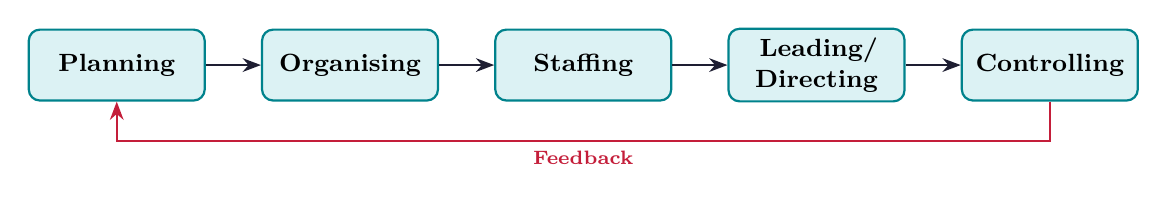
\begin{tikzpicture}[
  funcbox/.style={rectangle, draw=myteal, fill=hdrteal, text width=2.0cm,
    align=center, minimum height=0.9cm, font=\small\bfseries, rounded corners=4pt, line width=0.8pt},
  arrow/.style={-Stealth, thick, color=mydark}
]
  \node[funcbox] (plan) {Planning};
  \node[funcbox, right=0.7cm of plan] (org) {Organising};
  \node[funcbox, right=0.7cm of org] (staff) {Staffing};
  \node[funcbox, right=0.7cm of staff] (lead) {Leading/ Directing};
  \node[funcbox, right=0.7cm of lead] (ctrl) {Controlling};

  \draw[arrow] (plan) -- (org);
  \draw[arrow] (org)  -- (staff);
  \draw[arrow] (staff) -- (lead);
  \draw[arrow] (lead) -- (ctrl);
  \draw[redarrow] (ctrl.south) -- ++(0,-0.5) -| (plan.south)
    node[pos=0.25, below, font=\scriptsize\bfseries\color{myred}] {Feedback};
\end{tikzpicture}
\end{tcolorbox}

\begin{itemize}[leftmargin=*, itemsep=3pt]
  \item \textbf{Planning:} Deciding in advance what to do, how to do it, when to do it, and who is to do it. It bridges the gap between where we are and where we want to be.
  \item \textbf{Organising:} Arranging resources and tasks to achieve the plan. Involves grouping activities, assigning duties, and delegating authority.
  \item \textbf{Staffing:} Filling and keeping filled the positions in the organisation structure. Includes recruitment, selection, training, and development.
  \item \textbf{Leading/Directing:} Guiding and supervising subordinates to accomplish organisational goals. Involves communication, motivation, and leadership.
  \item \textbf{Controlling:} Measuring actual performance against planned targets and taking corrective action when necessary.
\end{itemize}

\subsection{Roles of a Manager}
Henry Mintzberg classified managerial roles into three categories based on his research on how managers actually spend their time. He identified \textbf{10 specific roles} grouped under Interpersonal, Informational, and Decisional categories. Unlike the classical view that managers only plan, organise, and control, Mintzberg showed that managerial work is varied, fragmented, and action-oriented. These roles are interlinked and a manager plays all of them simultaneously, with the emphasis shifting depending on the level and context.

\par\noindent
\begin{tabularx}{\linewidth}{|B{3.0cm}|Y|Y|}
\hline
\rowcolor{hdrgray}
\multicolumn{1}{|>{\centering\arraybackslash}m{3.0cm}|}{\textbf{Category}} &
\multicolumn{1}{>{\centering\arraybackslash}Y|}{\textbf{Role}} &
\multicolumn{1}{>{\centering\arraybackslash}Y|}{\textbf{Description}} \\
\hline
\multirow{3}{*}{\textbf{Interpersonal}} & Figurehead & Performs ceremonial duties (e.g., signing documents, representing the organisation). \\
\cline{2-3}
 & Leader & Motivates, directs, and coordinates the activities of subordinates. \\
\cline{2-3}
 & Liaison & Maintains networks with outsiders and peers for information and support. \\
\hline
\multirow{3}{*}{\textbf{Informational}} & Monitor & Scans internal and external environment for information. \\
\cline{2-3}
 & Disseminator & Transmits information received from outside to members of the organisation. \\
\cline{2-3}
 & Spokesperson & Transmits information to outsiders on the organisation's plans and policies. \\
\hline
\multirow{4}{*}{\textbf{Decisional}} & Entrepreneur & Initiates change; searches for new opportunities and improvement projects. \\
\cline{2-3}
 & Disturbance Handler & Takes corrective action when the organisation faces unexpected crises. \\
\cline{2-3}
 & Resource Allocator & Decides who gets resources --- time, money, equipment, and manpower. \\
\cline{2-3}
 & Negotiator & Represents the organisation in major negotiations with unions, suppliers, etc. \\
\hline
\end{tabularx}

\subsection{Levels of Management}
Management is typically divided into three hierarchical levels:

\begin{tcolorbox}[tikzbox, title={Levels of Management --- Hierarchy}]
\centering
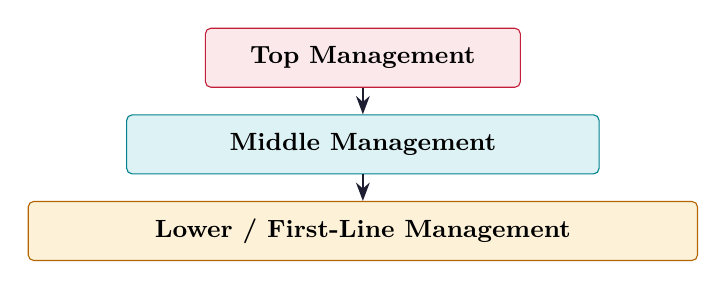
\begin{tikzpicture}
  \node[draw=myred, fill=hdrred, minimum width=4.0cm, minimum height=0.75cm,
    align=center, font=\small\bfseries, rounded corners=2pt] (top) at (0,0)
    {Top Management};
  \node[draw=myteal, fill=hdrteal, minimum width=6.0cm, minimum height=0.75cm,
    align=center, font=\small\bfseries, rounded corners=2pt] (mid) at (0,-1.1)
    {Middle Management};
  \node[draw=myamber, fill=hdramber, minimum width=8.5cm, minimum height=0.75cm,
    align=center, font=\small\bfseries, rounded corners=2pt] (low) at (0,-2.2)
    {Lower / First-Line Management};

  \draw[arrow] (top) -- (mid);
  \draw[arrow] (mid) -- (low);
\end{tikzpicture}
\end{tcolorbox}

\par\noindent
\begin{tabularx}{\linewidth}{|B{2.8cm}|Y|Y|}
\hline
\rowcolor{hdrgray}
\multicolumn{1}{|>{\centering\arraybackslash}m{2.8cm}|}{\textbf{Level}} &
\multicolumn{1}{>{\centering\arraybackslash}Y|}{\textbf{Examples}} &
\multicolumn{1}{>{\centering\arraybackslash}Y|}{\textbf{Key Activities}} \\
\hline
Top Management & CEO, MD, Board of Directors & Set overall strategy, goals, and policies; represent company externally. \\
\hline
Middle Management & Dept. Heads, Branch Managers, General Managers & Implement top-level strategies; coordinate lower-level activities. \\
\hline
First-Line Management & Supervisors, Foremen, Team Leaders & Direct and supervise operative employees; handle day-to-day operations. \\
\hline
\end{tabularx}

% ===============================================================================
\section{Functions of Management --- Planning}
% ===============================================================================

\begin{tcolorbox}[defbox, title={\textbf{Planning --- Definition}}]
\textbf{Planning} is the primary management function that involves setting objectives and determining the best course of action to achieve them. It is forward-looking, involves decision-making, and serves as the basis for all other management functions.
\end{tcolorbox}

\subsection{Concept and Nature of Planning}
\begin{itemize}[leftmargin=*, itemsep=3pt]
  \item \textbf{Purposeful:} Planning is always directed toward the achievement of specific goals.
  \item \textbf{Primary Function:} Planning precedes all other management functions --- organising, staffing, directing, and controlling all depend on planning.
  \item \textbf{Pervasive:} All managers at all levels engage in planning, though the scope and time horizon differ.
  \item \textbf{Future-Oriented:} Planning deals with predicting future conditions and preparing for them.
  \item \textbf{Decision-Making:} Planning involves making a choice among various alternative courses of action.
  \item \textbf{Continuous Process:} Plans are constantly reviewed and revised in response to changing conditions.
  \item \textbf{Mental Exercise:} Planning requires intelligence, foresight, imagination, and sound judgment.
\end{itemize}

\subsection{Types of Plans}
\par\noindent
\begin{tabularx}{\linewidth}{|B{3.0cm}|Y|Y|}
\hline
\rowcolor{myteal}
\multicolumn{1}{|>{\centering\arraybackslash\color{white}}m{3.0cm}|}{\textbf{Type}} &
\multicolumn{1}{>{\centering\arraybackslash\color{white}}Y|}{\textbf{Description}} &
\multicolumn{1}{>{\centering\arraybackslash\color{white}}Y|}{\textbf{Example}} \\
\hline
Mission/Purpose & Fundamental reason for the organisation's existence. & ``Provide affordable, clean energy to all.'' \\
\hline
Objectives/Goals & Specific, measurable targets to be achieved within a time frame. & Increase sales by 20\% in FY 2026. \\
\hline
Strategies & Long-term, broad plans to achieve objectives in a competitive environment. & Market penetration, diversification. \\
\hline
Policies & General guidelines that channel thinking and decision-making. & ``All employees must follow the safety code.'' \\
\hline
Procedures & Step-by-step sequences for handling recurring activities. & Leave application procedure. \\
\hline
Rules & Specific, definite actions or prohibitions with no discretion. & ``No smoking in office premises.'' \\
\hline
Programmes & Complex of goals, policies, procedures, and budgets for a major action. & Employee training programme. \\
\hline
Budgets & A plan expressed in numerical terms (usually money or units). & Annual capital expenditure budget. \\
\hline
\end{tabularx}

\subsection{Management by Objectives (MBO)}

\begin{tcolorbox}[defbox, title={\textbf{MBO --- Definition}}]
\textbf{Management by Objectives (MBO)}, developed by Peter Drucker (1954), is a management philosophy in which superiors and subordinates jointly identify common goals, define each individual's major areas of responsibility in terms of results expected, and use these measures as guides for operating the unit and assessing the contribution of its members.
\end{tcolorbox}

\subsubsection{Process of MBO}
\begin{enumerate}[label=\textbf{\arabic*.}, leftmargin=*, itemsep=3pt, topsep=2pt]
  \item \textbf{Set Organisational Objectives:} Top management defines long-term strategic goals.
  \item \textbf{Cascade Objectives:} Goals are broken down from organisation level to department level to individual level.
  \item \textbf{Participate in Goal-Setting:} Managers and subordinates jointly set individual performance objectives.
  \item \textbf{Monitor Progress:} Periodic reviews are held to assess progress against objectives.
  \item \textbf{Evaluate Performance:} At the end of the period, actual results are compared against objectives.
  \item \textbf{Provide Feedback and Rewards:} Employees receive feedback; rewards are linked to objective achievement.
\end{enumerate}

\subsubsection{Advantages and Disadvantages of MBO}
\par\noindent
\begin{tabularx}{\linewidth}{|Y|Y|}
\hline
\rowcolor{hdrgray}
\multicolumn{1}{|>{\centering\arraybackslash}Y|}{\textbf{Advantages}} &
\multicolumn{1}{>{\centering\arraybackslash}Y|}{\textbf{Disadvantages}} \\
\hline
Clarifies roles and responsibilities. & Time-consuming; requires extensive paperwork. \\
\hline
Improves motivation by involving employees. & Difficult to set verifiable, measurable objectives. \\
\hline
Facilitates performance appraisal. & May focus only on short-term quantitative goals. \\
\hline
Encourages participative management. & Fails if top management is not fully committed. \\
\hline
Improves planning and coordination. & Can create pressure and stress if goals are unrealistic. \\
\hline
\end{tabularx}

% ===============================================================================
\section{Organisation Structure}
% ===============================================================================

\begin{tcolorbox}[defbox, title={\textbf{Organisation --- Definition}}]
\textbf{Organisation} is the process of identifying and grouping work to be performed, defining and delegating responsibility and authority, and establishing relationships to enable people to work most effectively together in accomplishing objectives.
\end{tcolorbox}

\subsection{Principles of Organisation}
\begin{itemize}[leftmargin=*, itemsep=3pt]
  \item \textbf{Principle of Objective:} Every organisational unit and every activity must contribute to organisational objectives.
  \item \textbf{Principle of Unity of Objective:} The structure of the organisation must reflect and support the overall objective.
  \item \textbf{Principle of Division of Labour:} Work must be divided into specialised tasks to improve efficiency.
  \item \textbf{Principle of Authority and Responsibility:} Authority and responsibility must be clearly defined and commensurate with each other.
  \item \textbf{Unity of Command:} Each subordinate should receive orders from only one superior to avoid confusion.
  \item \textbf{Scalar Principle:} There must be a clear line of authority from the top to the bottom of the organisation.
  \item \textbf{Span of Management:} Each superior can effectively supervise only a limited number of subordinates.
  \item \textbf{Exception Principle:} Managers at higher levels should deal only with exceptional (non-routine) matters.
\end{itemize}

\subsection{Centralisation vs. Decentralisation}
\par\noindent
\begin{tabularx}{\linewidth}{|B{3.2cm}|Y|Y|}
\hline
\rowcolor{hdrgray}
\multicolumn{1}{|>{\centering\arraybackslash}m{3.2cm}|}{\textbf{Aspect}} &
\multicolumn{1}{>{\centering\arraybackslash}Y|}{\textbf{Centralisation}} &
\multicolumn{1}{>{\centering\arraybackslash}Y|}{\textbf{Decentralisation}} \\
\hline
Definition & Decision-making authority is concentrated at the top level of management. & Decision-making authority is distributed to lower levels of management. \\
\hline
Speed of Decision & Slow --- requires top management approval. & Fast --- decisions made at operational level. \\
\hline
Uniformity & High uniformity in policies and actions. & Less uniformity; more flexibility. \\
\hline
Motivation & Low --- subordinates have little autonomy. & High --- subordinates feel empowered. \\
\hline
Suitable for & Small organisations or crisis situations. & Large organisations or multi-location firms. \\
\hline
\end{tabularx}

\subsection{Span of Management}

\begin{tcolorbox}[defbox, title={\textbf{Span of Management}}]
\textbf{Span of Management} (also called Span of Control) refers to the number of subordinates a manager can effectively and efficiently supervise and direct. A \textbf{narrow span} results in a tall hierarchical structure; a \textbf{wide span} results in a flat structure.
\end{tcolorbox}

\textbf{Factors affecting Span of Management:}
\begin{itemize}[leftmargin=*, itemsep=2pt]
  \item Ability and competence of the manager and subordinates.
  \item Nature of the work (routine vs. complex).
  \item Degree of standardisation and delegation.
  \item Availability of communication technology and staff assistance.
  \item Geographic dispersion of subordinates.
\end{itemize}

\subsection{Organisational Effectiveness}

\begin{tcolorbox}[defbox, title={\textbf{Organisational Effectiveness}}]
\textbf{Organisational Effectiveness} is the degree to which an organisation achieves its goals and objectives using the available resources efficiently. It encompasses financial performance, stakeholder satisfaction, internal process quality, and capacity to adapt and learn.
\end{tcolorbox}

\textbf{Approaches to measuring Organisational Effectiveness:}
\begin{enumerate}[label=\textbf{\arabic*.}, leftmargin=*, itemsep=3pt, topsep=2pt]
  \item \textbf{Goal Attainment Approach:} Measures the extent to which stated goals are achieved (e.g., profit targets, production quotas).
  \item \textbf{Systems Resource Approach:} Focuses on the ability to acquire scarce and valued resources from the external environment.
  \item \textbf{Internal Process Approach:} Evaluates the health of internal operations (e.g., employee morale, communication, conflict resolution).
  \item \textbf{Strategic Constituencies Approach:} Assesses satisfaction of all key stakeholder groups (owners, employees, customers, suppliers, government).
\end{enumerate}

% ===============================================================================
% MANDATORY QUICK REVISION PAGE
% ===============================================================================
\newpage
\begin{center}
  {\large\bfseries\color{myred} Quick Revision --- Module 1}\\[3pt]
  {\small\color{mydark} Basic Concepts, Planning \& Organisation $|$ HS-HU701}
\end{center}
\noindent{\color{myred}\rule{\linewidth}{1.2pt}}
\vspace{4pt}

\begin{tcolorbox}[formulabox, title={\textbf{Key Concepts at a Glance}}]
\renewcommand{\arraystretch}{1.3}
\begin{tabularx}{\linewidth}{B{4.0cm} X}
Management & Planning + Organising + Staffing + Leading + Controlling \\[3pt]
Efficiency & Doing things \textbf{right} (minimising waste) \\[3pt]
Effectiveness & Doing the \textbf{right things} (achieving goals) \\[3pt]
MBO & Joint goal-setting by superiors and subordinates \\[3pt]
Unity of Command & One subordinate $\rightarrow$ one superior \\[3pt]
Span of Management & No.\ of subordinates a manager can effectively supervise \\[3pt]
Centralisation & Decision power at top; Decentralisation = power distributed downward \\
\end{tabularx}
\end{tcolorbox}

\begin{tcolorbox}[defbox, title={\textbf{One-Line Definitions}}]
\begin{itemize}[leftmargin=*, itemsep=2pt, topsep=0pt]
  \item \textbf{Management:} Process of planning, organising, staffing, leading, and controlling to achieve organisational goals.
  \item \textbf{Planning:} Deciding in advance what to do, how, when, and by whom.
  \item \textbf{Organising:} Grouping tasks and assigning responsibilities and authority to achieve the plan.
  \item \textbf{Staffing:} Filling and maintaining positions in the organisational structure.
  \item \textbf{Leading:} Guiding and influencing people to achieve goals (motivation + communication).
  \item \textbf{Controlling:} Comparing actual performance with standards and taking corrective action.
  \item \textbf{MBO:} Management philosophy where managers and subordinates jointly set measurable goals.
  \item \textbf{Scalar Chain:} Clear line of authority from highest to lowest level in an organisation.
  \item \textbf{Organisational Effectiveness:} Degree to which an organisation achieves its goals using available resources.
\end{itemize}
\end{tcolorbox}

\begin{tcolorbox}[exambox, title={\textbf{Frequently Asked / Viva Questions}}]
\begin{enumerate}[topsep=0pt, label=\textbf{Q\arabic*.}, itemsep=5pt]
  \item \Q{Define management. What is the difference between efficiency and effectiveness?}
    Management is the process of coordinating resources to achieve goals. Efficiency means doing things right with minimum waste; effectiveness means doing the right things to achieve desired outcomes.
  \item \Q{List the five functions of management in sequence.}
    Planning $\rightarrow$ Organising $\rightarrow$ Staffing $\rightarrow$ Leading/Directing $\rightarrow$ Controlling.
  \item \Q{What are Henry Mintzberg's three categories of managerial roles?}
    Interpersonal (Figurehead, Leader, Liaison), Informational (Monitor, Disseminator, Spokesperson), and Decisional (Entrepreneur, Disturbance Handler, Resource Allocator, Negotiator).
  \item \Q{What are the three levels of management? Give one example of each.}
    Top level (CEO), Middle level (Department Manager), First-line/Lower level (Supervisor or Foreman).
  \item \Q{What is the nature of planning? Why is it considered the primary management function?}
    Planning is goal-oriented, future-oriented, and involves decision-making. It is primary because all other functions --- organising, staffing, leading, and controlling --- depend on the plans that are made.
  \item \Q{What is Management by Objectives (MBO)? Who developed it?}
    MBO, developed by Peter Drucker (1954), is a process where superiors and subordinates jointly identify goals, define areas of responsibility, and use these as guides for performance evaluation.
  \item \Q{What is the principle of Unity of Command?}
    Each subordinate should receive orders and instructions from only one superior to avoid conflicting directives and confusion.
  \item \Q{Distinguish between centralisation and decentralisation.}
    Centralisation concentrates decision-making authority at the top management level for uniformity and control. Decentralisation distributes authority to lower levels for faster decisions and greater employee motivation.
  \item \Q{What is Span of Management (Span of Control)? What factors affect it?}
    It is the number of subordinates a manager can effectively supervise. It is affected by the manager's ability, complexity of work, degree of standardisation, communication technology, and geographic dispersion of staff.
  \item \Q{What is organisational effectiveness? Name two approaches to measure it.}
    It is the degree to which an organisation achieves its goals efficiently. Two approaches: Goal Attainment Approach (measuring achievement of stated goals) and Strategic Constituencies Approach (measuring stakeholder satisfaction).
  \item \Q{What are the key advantages of MBO?}
    MBO clarifies roles, improves motivation through participation, facilitates objective performance appraisal, and improves overall planning and coordination.
  \item \Q{Differentiate between policies and rules in planning.}
    Policies are broad guidelines that channel decision-making (e.g., ``Promote from within''); rules are specific mandatory directives with no discretion (e.g., ``No smoking on premises'').
\end{enumerate}
\end{tcolorbox}

\begin{tcolorbox}[tikzbox, title={Management Levels vs.\ Skills Required}]
\centering
\renewcommand{\arraystretch}{1.4}
\begin{tabularx}{\linewidth}{|B{3.0cm}|Y|Y|Y|}
\hline
\rowcolor{hdrgray}
\multicolumn{1}{|>{\centering\arraybackslash}m{3.0cm}|}{\textbf{Level}} &
\multicolumn{1}{>{\centering\arraybackslash}Y|}{\textbf{Conceptual Skills}} &
\multicolumn{1}{>{\centering\arraybackslash}Y|}{\textbf{Human Skills}} &
\multicolumn{1}{>{\centering\arraybackslash}Y|}{\textbf{Technical Skills}} \\
\hline
Top Management & High & Medium & Low \\
\hline
Middle Management & Medium & High & Medium \\
\hline
First-Line Management & Low & Medium & High \\
\hline
\end{tabularx}
\end{tcolorbox}


% -- Module 2 -----------------------------------------------------------------
\modulestart{2}{Management and Society}

\section{Management and Society}
% ===============================================================================

\begin{tcolorbox}[defbox, title={\textbf{Management and Society --- Overview}}]
\textbf{Management and Society} refers to the interdependent relationship between organisations and their social environment. Modern organisations are not isolated entities; they are open systems embedded within society and are affected by social, political, legal, and economic forces --- and, in turn, they affect society.
\end{tcolorbox}

\subsection{External Environment of an Organisation}
The external environment consists of all forces outside the organisation that can influence its performance:

\begin{tcolorbox}[tikzbox, title={External Environment of an Organisation}]
\centering
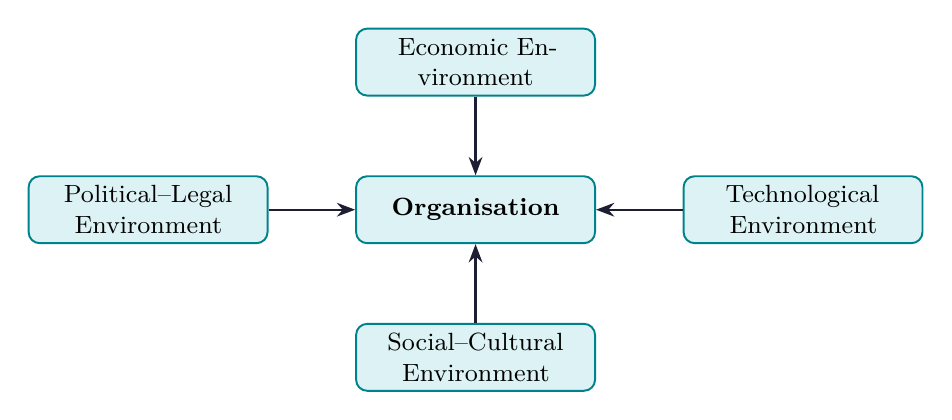
\begin{tikzpicture}[
  envbox/.style={rectangle, draw=myteal, fill=hdrteal, text width=2.8cm,
    align=center, minimum height=0.85cm, font=\small, rounded corners=4pt, line width=0.7pt},
  arrow/.style={-Stealth, thick, color=mydark}
]
  \node[envbox] (org) at (0,0) {\textbf{Organisation}};
  \node[envbox, above=1.0cm of org] (eco) {Economic Environment};
  \node[envbox, right=1.1cm of org] (tech) {Technological Environment};
  \node[envbox, below=1.0cm of org] (soc) {Social--Cultural Environment};
  \node[envbox, left=1.1cm of org] (pol) {Political--Legal Environment};

  \draw[arrow] (eco) -- (org);
  \draw[arrow] (tech) -- (org);
  \draw[arrow] (soc) -- (org);
  \draw[arrow] (pol) -- (org);
\end{tikzpicture}
\end{tcolorbox}

\begin{itemize}[leftmargin=*, itemsep=3pt]
  \item \textbf{Economic Environment:} Includes inflation, interest rates, GDP growth, unemployment levels, and business cycles. Directly affects demand, costs, and investment decisions.
  \item \textbf{Technological Environment:} Pace of innovation, automation, R\&D, and digitisation. Affects production methods, products, and competitive advantage.
  \item \textbf{Social--Cultural Environment:} Demographics, lifestyle changes, cultural values, education levels, and social norms. Affects consumer behaviour and workforce composition.
  \item \textbf{Political--Legal Environment:} Government stability, taxation policy, labour laws, environmental regulations, and trade policies. Shapes the rules within which organisations operate.
  \item \textbf{Natural Environment:} Availability of natural resources, environmental sustainability concerns, climate regulations.
\end{itemize}

\subsection{Corporate Social Responsibility (CSR)}

\begin{tcolorbox}[defbox, title={\textbf{Corporate Social Responsibility (CSR)}}]
\textbf{CSR} is the obligation of business organisations to act in ways that protect and improve the welfare of society along with their own interests. It represents a company's commitment to operating in an economically, socially, and environmentally responsible manner beyond what the law requires.
\end{tcolorbox}

\subsubsection{Carroll's Pyramid of CSR}
Carroll (1991) proposed four layers of corporate responsibility, from the most fundamental to the most discretionary:

\begin{tcolorbox}[tikzbox, title={Carroll's Pyramid of CSR}]
\centering
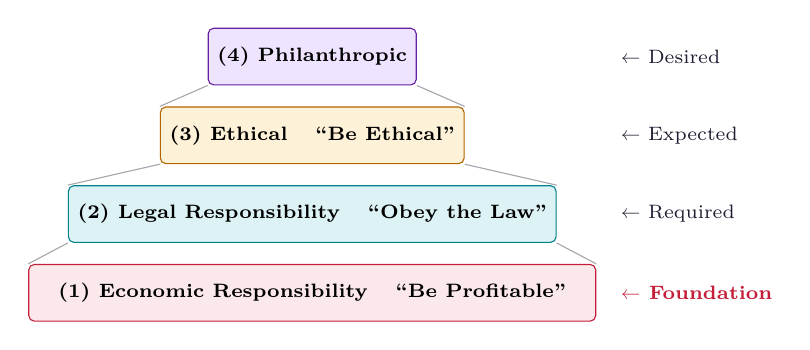
\begin{tikzpicture}[every node/.style={align=center}]
  % Pyramid layers — bottom (widest) to top (narrowest), centered at x=0
  % Each layer: box on left, label on right (with enough offset)
  \node[draw=myred, fill=hdrred, minimum width=7.2cm, minimum height=0.72cm,
    font=\scriptsize\bfseries, rounded corners=2pt] (eco) at (0, 0)
    {(1) Economic Responsibility \quad ``Be Profitable''};

  \node[draw=myteal, fill=hdrteal, minimum width=5.4cm, minimum height=0.72cm,
    font=\scriptsize\bfseries, rounded corners=2pt] (leg) at (0, 1.0)
    {(2) Legal Responsibility \quad ``Obey the Law''};

  \node[draw=myamber, fill=hdramber, minimum width=3.6cm, minimum height=0.72cm,
    font=\scriptsize\bfseries, rounded corners=2pt] (eth) at (0, 2.0)
    {(3) Ethical \quad ``Be Ethical''};

  \node[draw=mypurple, fill=hdrpurple, minimum width=1.8cm, minimum height=0.72cm,
    font=\scriptsize\bfseries, rounded corners=2pt] (phi) at (0, 3.0)
    {(4) Philanthropic};

  % Right-side labels placed well clear of the boxes
  \node[font=\scriptsize\bfseries\color{myred},   anchor=west] at (3.8, 0)   {$\leftarrow$ Foundation};
  \node[font=\scriptsize\color{mydark},            anchor=west] at (3.8, 1.0) {$\leftarrow$ Required};
  \node[font=\scriptsize\color{mydark},            anchor=west] at (3.8, 2.0) {$\leftarrow$ Expected};
  \node[font=\scriptsize\color{mydark},            anchor=west] at (3.8, 3.0) {$\leftarrow$ Desired};

  % Connecting lines between layers to show pyramid structure
  \draw[mydark!40, thin] (eco.north west) -- (leg.south west);
  \draw[mydark!40, thin] (eco.north east) -- (leg.south east);
  \draw[mydark!40, thin] (leg.north west) -- (eth.south west);
  \draw[mydark!40, thin] (leg.north east) -- (eth.south east);
  \draw[mydark!40, thin] (eth.north west) -- (phi.south west);
  \draw[mydark!40, thin] (eth.north east) -- (phi.south east);
\end{tikzpicture}
\end{tcolorbox}

\subsubsection{Arguments For and Against CSR}
\par\noindent
\begin{tabularx}{\linewidth}{|Y|Y|}
\hline
\rowcolor{hdrgray}
\multicolumn{1}{|>{\centering\arraybackslash}Y|}{\textbf{Arguments For CSR}} &
\multicolumn{1}{>{\centering\arraybackslash}Y|}{\textbf{Arguments Against CSR}} \\
\hline
Improves brand image and public trust. & Increases costs and reduces profitability. \\
\hline
Attracts socially conscious investors and customers. & Management's primary duty is profit maximisation (Friedman doctrine). \\
\hline
Reduces regulatory scrutiny and legal risk. & Dilutes focus from core business competence. \\
\hline
Enhances employee motivation and retention. & Can lead to misuse of corporate funds. \\
\hline
Contributes to long-term sustainable development. & Difficult to measure the return on CSR investment. \\
\hline
\end{tabularx}

\subsection{Corporate Governance}

\begin{tcolorbox}[defbox, title={\textbf{Corporate Governance}}]
\textbf{Corporate Governance} refers to the system of rules, practices, and processes by which a company is directed and controlled. It balances the interests of a company's many stakeholders --- shareholders, management, customers, suppliers, financiers, government, and the community.
\end{tcolorbox}

\textbf{Key principles of Good Corporate Governance:}
\begin{itemize}[leftmargin=*, itemsep=2pt]
  \item \textbf{Accountability:} Directors and management are accountable to shareholders.
  \item \textbf{Transparency:} Full, accurate, and timely disclosure of financial and non-financial information.
  \item \textbf{Fairness:} Equal treatment of all shareholders, including minority shareholders.
  \item \textbf{Responsibility:} Management must act responsibly toward all stakeholders.
  \item \textbf{Independence:} Independent board members free from management influence.
\end{itemize}

\subsection{Ethical Standards in Management}

\begin{tcolorbox}[defbox, title={\textbf{Business Ethics}}]
\textbf{Business Ethics} refers to the application of ethical principles and moral standards to business activities, relationships, and decisions. It involves distinguishing between right and wrong conduct in the workplace.
\end{tcolorbox}

\textbf{Sources of unethical behaviour in organisations:}
\begin{itemize}[leftmargin=*, itemsep=2pt]
  \item Excessive pressure to meet short-term financial targets.
  \item Ambiguous or absent codes of conduct.
  \item Weak enforcement of ethical standards by top management.
  \item Peer pressure and cultural normalisation of unethical acts.
\end{itemize}

\textbf{How to improve ethical standards:}
\begin{itemize}[leftmargin=*, itemsep=2pt]
  \item Develop and communicate a formal Code of Ethics.
  \item Lead by example --- ethical behaviour from top management.
  \item Establish whistleblower protection mechanisms.
  \item Conduct regular ethics training programmes.
  \item Include ethical criteria in performance appraisal.
\end{itemize}

% ===============================================================================
\section{People Management}
% ===============================================================================

\begin{tcolorbox}[defbox, title={\textbf{People Management --- Overview}}]
\textbf{People Management} (Human Resource Management) involves planning for, acquiring, developing, and retaining people in an organisation so that they contribute maximally to organisational goals.
\end{tcolorbox}

\subsection{Job Design}

\begin{tcolorbox}[defbox, title={\textbf{Job Design}}]
\textbf{Job Design} is the process of organising tasks, duties, and responsibilities into a productive unit of work. It defines the content and method of a job and influences employee motivation, satisfaction, and productivity.
\end{tcolorbox}

\textbf{Major approaches to job design:}
\begin{enumerate}[label=\textbf{\arabic*.}, leftmargin=*, itemsep=3pt, topsep=2pt]
  \item \textbf{Job Simplification:} Breaking jobs into small, repetitive, standardised tasks. Maximises efficiency but may cause boredom (Taylor's Scientific Management approach).
  \item \textbf{Job Rotation:} Systematically moving employees across different jobs or departments. Reduces boredom and builds versatility.
  \item \textbf{Job Enlargement:} Adding more tasks of similar complexity to a job (horizontal expansion) to increase variety.
  \item \textbf{Job Enrichment:} Adding more responsibility, autonomy, and complexity to a job (vertical expansion). Based on Herzberg's two-factor theory --- enhances motivation.
\end{enumerate}

\textbf{Hackman and Oldham's Job Characteristics Model} identifies five core dimensions:
\begin{itemize}[leftmargin=*, itemsep=2pt]
  \item \textbf{Skill variety:} Degree to which a job requires different skills and talents.
  \item \textbf{Task identity:} Degree to which the job involves doing a complete piece of work.
  \item \textbf{Task significance:} Degree to which the job has a substantial impact on others.
  \item \textbf{Autonomy:} Degree to which the job provides freedom and independence.
  \item \textbf{Feedback:} Degree to which the job itself provides direct performance information.
\end{itemize}

\subsection{Recruitment and Selection}

\begin{tcolorbox}[defbox, title={\textbf{Recruitment and Selection}}]
\textbf{Recruitment} is the process of attracting qualified candidates for job vacancies. \textbf{Selection} is the process of choosing the most suitable candidate from the pool of recruited applicants.
\end{tcolorbox}

\par\noindent
\begin{tabularx}{\linewidth}{|B{3.0cm}|Y|Y|}
\hline
\rowcolor{hdrgray}
\multicolumn{1}{|>{\centering\arraybackslash}m{3.0cm}|}{\textbf{Aspect}} &
\multicolumn{1}{>{\centering\arraybackslash}Y|}{\textbf{Recruitment}} &
\multicolumn{1}{>{\centering\arraybackslash}Y|}{\textbf{Selection}} \\
\hline
Definition & Attracting a pool of qualified applicants. & Choosing the best fit from the applicants. \\
\hline
Nature & Positive process (attract more applicants). & Negative process (eliminate unsuitable candidates). \\
\hline
Outcome & Pool of candidates. & Single best candidate appointed. \\
\hline
Sources & Internal (promotions, transfers) or External (ads, job fairs, campus). & Interviews, tests, background checks. \\
\hline
\end{tabularx}

\subsection{Training and Development}

\begin{tcolorbox}[defbox, title={\textbf{Training vs.\ Development}}]
\textbf{Training} is a short-term, systematic process that improves employees' specific job-related skills and knowledge for their current role.
\par\vspace{3pt}
\textbf{Development} is a long-term process aimed at improving the overall capabilities and career growth of employees for future roles.
\end{tcolorbox}

\textbf{Common training methods:}
\begin{itemize}[leftmargin=*, itemsep=2pt]
  \item \textbf{On-the-Job Training (OJT):} Apprenticeship, coaching, mentoring, job rotation.
  \item \textbf{Off-the-Job Training:} Lectures, case studies, simulations, vestibule training, role-playing.
  \item \textbf{E-Learning:} Online courses, virtual classrooms, webinars.
\end{itemize}

\subsection{Stress Management}

\begin{tcolorbox}[defbox, title={\textbf{Stress in the Workplace}}]
\textbf{Stress} is the physical and emotional response to excessive demands or pressures that exceed a person's ability to cope. Moderate stress (eustress) can improve performance, but chronic stress (distress) reduces productivity and health.
\end{tcolorbox}

\textbf{Common causes of workplace stress (stressors):}
\begin{itemize}[leftmargin=*, itemsep=2pt]
  \item Work overload, unrealistic deadlines, and poor time management.
  \item Role ambiguity (unclear responsibilities) or role conflict (conflicting demands).
  \item Poor relationships with supervisors or colleagues.
  \item Job insecurity and lack of career growth opportunities.
  \item Physical conditions: noise, poor lighting, and uncomfortable workspace.
\end{itemize}

\textbf{Stress management strategies:}
\par\noindent
\begin{tabularx}{\linewidth}{|B{3.2cm}|Y|}
\hline
\rowcolor{myteal}
\multicolumn{1}{|>{\centering\arraybackslash\color{white}}m{3.2cm}|}{\textbf{Approach}} &
\multicolumn{1}{>{\centering\arraybackslash\color{white}}Y|}{\textbf{Methods}} \\
\hline
Individual (employee) & Time management, exercise, relaxation techniques, social support. \\
\hline
Organisational & Clear role definitions, flexible work arrangements, counselling programmes, realistic goal-setting. \\
\hline
Job Redesign & Reducing overload; increasing autonomy and feedback. \\
\hline
\end{tabularx}

% ===============================================================================
\section{Managerial Competencies}
% ===============================================================================

\subsection{Communication in Management}

\begin{tcolorbox}[defbox, title={\textbf{Communication --- Definition}}]
\textbf{Communication} is the process of transmitting information, ideas, thoughts, feelings, and emotions from one person to another through verbal, non-verbal, or written channels. Effective communication is essential for coordination, motivation, and decision-making.
\end{tcolorbox}

\textbf{Types of communication in an organisation:}
\begin{itemize}[leftmargin=*, itemsep=2pt]
  \item \textbf{Downward:} From higher to lower levels (orders, policies, instructions).
  \item \textbf{Upward:} From lower to higher levels (reports, feedback, grievances).
  \item \textbf{Horizontal/Lateral:} Among peers at the same level (coordination).
  \item \textbf{Diagonal:} Across different levels and departments (cross-functional teams).
  \item \textbf{Grapevine (Informal):} Unofficial communication networks; fast but often inaccurate.
\end{itemize}

\textbf{Barriers to effective communication:}
\begin{itemize}[leftmargin=*, itemsep=2pt]
  \item Physical barriers (noise, distance), Semantic barriers (jargon, language differences).
  \item Psychological barriers (perceptual biases, emotional state).
  \item Organisational barriers (rigid hierarchies, information overload).
\end{itemize}

\subsection{Motivation}

\begin{tcolorbox}[defbox, title={\textbf{Motivation --- Definition}}]
\textbf{Motivation} is the process that initiates, guides, and sustains goal-oriented behaviours. It is the internal force that drives an individual to take action, maintain effort, and persist toward a goal.
\end{tcolorbox}

\textbf{Major motivation theories:}

\par\noindent
\begin{tabularx}{\linewidth}{|B{3.5cm}|Y|}
\hline
\rowcolor{hdrgray}
\multicolumn{1}{|>{\centering\arraybackslash}m{3.5cm}|}{\textbf{Theory}} &
\multicolumn{1}{>{\centering\arraybackslash}Y|}{\textbf{Key Concept}} \\
\hline
Maslow's Hierarchy of Needs & Five levels: Physiological $\to$ Safety $\to$ Social $\to$ Esteem $\to$ Self-Actualisation. People are motivated to fulfil unmet needs. \\
\hline
Herzberg's Two-Factor Theory & \textbf{Hygiene factors} (salary, job security) prevent dissatisfaction. \textbf{Motivators} (achievement, recognition) create satisfaction. \\
\hline
McGregor's Theory X and Y & Theory X: Workers are lazy and need control. Theory Y: Workers are self-motivated and seek responsibility. \\
\hline
Vroom's Expectancy Theory & Motivation $=$ Expectancy $\times$ Instrumentality $\times$ Valence. Effort leads to performance, performance leads to outcome. \\
\hline
\end{tabularx}

\subsection{Team Effectiveness}

\begin{tcolorbox}[defbox, title={\textbf{Team vs.\ Group}}]
A \textbf{Group} is a collection of individuals who interact primarily to share information and make decisions. A \textbf{Team} is a small number of people with complementary skills who are committed to a common purpose, performance goals, and approach for which they hold themselves mutually accountable.
\end{tcolorbox}

\textbf{Tuckman's Stages of Team Development:}
\begin{enumerate}[label=\textbf{\arabic*.}, leftmargin=*, itemsep=2pt, topsep=2pt]
  \item \textbf{Forming:} Team members are introduced; roles and goals are unclear; polite and cautious behaviour.
  \item \textbf{Storming:} Conflict and competition arise as individual personalities emerge; power struggles.
  \item \textbf{Norming:} Team establishes norms, roles become clear, cohesion builds.
  \item \textbf{Performing:} Team works productively and cooperatively toward goals.
  \item \textbf{Adjourning:} Team disbands after goal achievement; members reflect on accomplishments.
\end{enumerate}

\subsection{Conflict Management}

\begin{tcolorbox}[defbox, title={\textbf{Conflict in Organisations}}]
\textbf{Conflict} is a disagreement between two or more parties over incompatible goals, limited resources, or differences in values and perceptions. Conflict can be \textbf{functional} (stimulates creativity and debate) or \textbf{dysfunctional} (destroys cohesion and performance).
\end{tcolorbox}

\textbf{Thomas--Kilmann Conflict Resolution Styles:}
\par\noindent
\begin{tabularx}{\linewidth}{|B{2.8cm}|Y|Y|}
\hline
\rowcolor{hdrgray}
\multicolumn{1}{|>{\centering\arraybackslash}m{2.8cm}|}{\textbf{Style}} &
\multicolumn{1}{>{\centering\arraybackslash}Y|}{\textbf{Description}} &
\multicolumn{1}{>{\centering\arraybackslash}Y|}{\textbf{When to Use}} \\
\hline
Competing & Assert own position; win--lose approach. & Emergencies; unpopular decisions. \\
\hline
Collaborating & Win--win; both parties work together to find a mutually satisfying solution. & Complex issues; long-term relationships. \\
\hline
Compromising & Each party gives up something; middle-ground solution. & Time pressure; equal-power parties. \\
\hline
Avoiding & Withdraw or postpone the conflict. & Trivial issues; when time is needed to cool down. \\
\hline
Accommodating & Yield to the other party; lose--win. & When preserving relationship is more important than outcome. \\
\hline
\end{tabularx}

\subsection{Creativity and Entrepreneurship}

\begin{tcolorbox}[defbox, title={\textbf{Creativity and Entrepreneurship}}]
\textbf{Creativity} is the ability to generate novel and useful ideas. \textbf{Entrepreneurship} is the process of identifying business opportunities and organising resources to exploit them, while accepting the associated risks.
\par\vspace{3pt}
\textbf{Intrapreneurship:} Entrepreneurial behaviour within an existing organisation --- employees act as internal entrepreneurs to develop new products or processes.
\end{tcolorbox}

\textbf{Characteristics of creative/entrepreneurial managers:}
\begin{itemize}[leftmargin=*, itemsep=2pt]
  \item High tolerance for ambiguity and risk.
  \item Intrinsic motivation and persistent problem-solving drive.
  \item Ability to connect disparate ideas and synthesise novel solutions.
  \item Strong networking and resource-mobilisation skills.
\end{itemize}

% ===============================================================================
% MANDATORY QUICK REVISION PAGE
% ===============================================================================
\newpage
\begin{center}
  {\large\bfseries\color{myred} Quick Revision --- Module 2}\\[3pt]
  {\small\color{mydark} Society, People Management \& Managerial Competencies $|$ HS-HU701}
\end{center}
\noindent{\color{myred}\rule{\linewidth}{1.2pt}}
\vspace{4pt}

\begin{tcolorbox}[formulabox, title={\textbf{Key Frameworks at a Glance}}]
\renewcommand{\arraystretch}{1.3}
\begin{tabularx}{\linewidth}{B{4.0cm} X}
Carroll's CSR Pyramid & Economic $\to$ Legal $\to$ Ethical $\to$ Philanthropic \\[3pt]
Job Enrichment & Vertical job expansion; adds autonomy and responsibility. \\[3pt]
Vroom's Expectancy & Motivation $=$ Expectancy $\times$ Instrumentality $\times$ Valence \\[3pt]
Tuckman's Team Stages & Forming $\to$ Storming $\to$ Norming $\to$ Performing $\to$ Adjourning \\[3pt]
Thomas--Kilmann & 5 conflict styles: Competing, Collaborating, Compromising, Avoiding, Accommodating \\
\end{tabularx}
\end{tcolorbox}

\begin{tcolorbox}[defbox, title={\textbf{One-Line Definitions}}]
\begin{itemize}[leftmargin=*, itemsep=2pt, topsep=0pt]
  \item \textbf{CSR:} Obligation of organisations to operate in a socially and environmentally responsible manner beyond legal requirements.
  \item \textbf{Corporate Governance:} System of rules and processes by which a company is directed and controlled.
  \item \textbf{Business Ethics:} Application of moral standards to business activities and decisions.
  \item \textbf{Job Design:} Organising tasks and responsibilities into a productive unit of work.
  \item \textbf{Job Enrichment:} Vertical expansion of a job by adding responsibility and autonomy.
  \item \textbf{Recruitment:} Process of attracting qualified candidates for vacancies (positive process).
  \item \textbf{Selection:} Process of choosing the best fit from recruited candidates (negative/elimination process).
  \item \textbf{Stress:} Emotional/physical response when demands exceed coping capacity.
  \item \textbf{Motivation:} Internal force that drives behaviour toward a goal.
  \item \textbf{Team:} Small group with complementary skills, shared goals, and mutual accountability.
  \item \textbf{Conflict:} Disagreement over incompatible goals, resources, or values.
  \item \textbf{Entrepreneurship:} Identifying opportunities and organising resources to exploit them while accepting risk.
\end{itemize}
\end{tcolorbox}

\begin{tcolorbox}[exambox, title={\textbf{Frequently Asked / Viva Questions}}]
\begin{enumerate}[topsep=0pt, label=\textbf{Q\arabic*.}, itemsep=5pt]
  \item \Q{What is CSR? What are Carroll's four levels of CSR?}
    CSR is a firm's commitment to act ethically and contribute to economic development while improving the quality of life. Carroll's four levels are: Economic (be profitable), Legal (obey the law), Ethical (be ethical), and Philanthropic (be a good citizen).
  \item \Q{What is Corporate Governance? Why is it important?}
    Corporate governance is the system of rules directing and controlling a company. It ensures accountability, transparency, and fair treatment of all stakeholders, preventing fraud and mismanagement.
  \item \Q{Distinguish between job enrichment and job enlargement.}
    Job enrichment adds more responsibility, autonomy, and complexity (vertical expansion). Job enlargement adds more tasks of similar difficulty (horizontal expansion). Enrichment is more motivating.
  \item \Q{What is Tuckman's model of team development? Name the five stages.}
    Tuckman's model describes team evolution through: Forming (polite, uncertain), Storming (conflict), Norming (cohesion), Performing (productive), and Adjourning (disbanding).
  \item \Q{State Herzberg's Two-Factor Theory. How does it differ from Maslow's theory?}
    Herzberg identifies Hygiene Factors (prevent dissatisfaction: salary, working conditions) and Motivators (create satisfaction: achievement, recognition). Unlike Maslow's single hierarchy, Herzberg separates dissatisfaction and satisfaction as two independent dimensions.
  \item \Q{What is Vroom's Expectancy Theory of motivation?}
    Motivation = Expectancy (effort will lead to performance) $\times$ Instrumentality (performance will lead to reward) $\times$ Valence (reward is valued). All three must be high for strong motivation.
  \item \Q{What are the five Thomas--Kilmann conflict resolution styles?}
    Competing (win--lose), Collaborating (win--win), Compromising (mutual concessions), Avoiding (withdraw), and Accommodating (yield to other party).
  \item \Q{What is the difference between recruitment and selection?}
    Recruitment is a positive process of attracting a pool of candidates; selection is a negative process of eliminating unsuitable candidates to choose the best fit.
  \item \Q{What are the main causes of workplace stress?}
    Work overload, role ambiguity, role conflict, poor superior relationships, job insecurity, and poor physical working conditions.
  \item \Q{What is intrapreneurship?}
    Intrapreneurship is entrepreneurial behaviour displayed by employees within an existing organisation --- acting like internal entrepreneurs to innovate, develop new products, or improve processes.
  \item \Q{Name the five core dimensions of Hackman and Oldham's Job Characteristics Model.}
    Skill variety, Task identity, Task significance, Autonomy, and Feedback.
  \item \Q{What are the key barriers to effective communication in an organisation?}
    Physical barriers (noise), Semantic barriers (language/jargon), Psychological barriers (bias, emotions), and Organisational barriers (hierarchy, information overload).
\end{enumerate}
\end{tcolorbox}

\begin{tcolorbox}[tikzbox, title={Training vs.\ Development --- Comparison}]
\centering
\renewcommand{\arraystretch}{1.4}
\begin{tabularx}{\linewidth}{|B{3.0cm}|Y|Y|}
\hline
\rowcolor{hdrgray}
\multicolumn{1}{|>{\centering\arraybackslash}m{3.0cm}|}{\textbf{Aspect}} &
\multicolumn{1}{>{\centering\arraybackslash}Y|}{\textbf{Training}} &
\multicolumn{1}{>{\centering\arraybackslash}Y|}{\textbf{Development}} \\
\hline
Time Horizon & Short-term & Long-term \\
\hline
Focus & Current job role & Future roles and career growth \\
\hline
Scope & Specific skills and knowledge & Broad capabilities and personality \\
\hline
Initiative & Organisation-driven & Individual and organisation \\
\hline
Example & Safety training, software training & Leadership development, MBA sponsorship \\
\hline
\end{tabularx}
\end{tcolorbox}


% -- Module 3 -----------------------------------------------------------------
\modulestart{3}{Leadership}

\section{Leadership}
% ===============================================================================

\begin{tcolorbox}[defbox, title={\textbf{Leadership --- Definition}}]
\textbf{Leadership} is the ability to influence, inspire, and guide others toward the achievement of organisational goals. A leader motivates followers to willingly exert effort toward common objectives.
\par\vspace{3pt}
\textbf{Manager vs.\ Leader:} A manager is appointed (formal authority); a leader may be formal or informal. Managers administer; leaders innovate. Managers maintain; leaders develop.
\end{tcolorbox}

\subsection{Concept and Nature of Leadership}
\begin{itemize}[leftmargin=*, itemsep=3pt]
  \item Leadership is a process, not just a position or trait.
  \item It involves a triad: \textbf{leader}, \textbf{followers}, and \textbf{situational context}.
  \item Effective leaders adapt their style to the readiness and needs of followers.
  \item Leadership is forward-looking; it involves creating a vision and aligning people toward it.
\end{itemize}

\subsection{Leadership Styles}

\par\noindent
\begin{tabularx}{\linewidth}{|B{3.0cm}|Y|Y|}
\hline
\rowcolor{hdrgray}
\multicolumn{1}{|>{\centering\arraybackslash}m{3.0cm}|}{\textbf{Style}} &
\multicolumn{1}{>{\centering\arraybackslash}Y|}{\textbf{Description}} &
\multicolumn{1}{>{\centering\arraybackslash}Y|}{\textbf{Best Suited For}} \\
\hline
Autocratic & Leader makes all decisions alone; high control, low participation. & Crises, unskilled workers, urgent tasks. \\
\hline
Democratic / Participative & Leader involves team in decision-making; shares authority. & Skilled/experienced teams; creative tasks. \\
\hline
Laissez-Faire / Free-Rein & Leader delegates fully; minimal intervention. & Highly skilled experts; research teams. \\
\hline
Transformational & Leader inspires change through vision, charisma, and individual attention. & Organisational change; long-term innovation. \\
\hline
Transactional & Leader motivates through reward and punishment; maintains the status quo. & Routine, well-defined tasks. \\
\hline
Servant Leadership & Leader prioritises the needs of followers; facilitates growth and well-being. & Service-oriented organisations, NGOs. \\
\hline
\end{tabularx}

\subsection{Key Leadership Theories}

\subsubsection{Trait Theory}
Leadership is determined by inherent personal qualities --- physical, mental, and personality characteristics. Key traits identified: intelligence, self-confidence, integrity, decisiveness, drive, and sociability.
\par\vspace{3pt}
\textbf{Limitation:} Does not explain why people with the same traits succeed in some situations and fail in others.

\subsubsection{Behavioural Theories}
Focus on what leaders \textit{do} rather than what they \textit{are}:
\begin{itemize}[leftmargin=*, itemsep=2pt]
  \item \textbf{Ohio State Studies:} Two dimensions --- \textbf{Initiating Structure} (task-oriented) and \textbf{Consideration} (people-oriented). Best leaders are high on both.
  \item \textbf{Michigan Studies:} \textbf{Production-centred} vs.\ \textbf{Employee-centred} leadership. Employee-centred leaders achieve higher productivity and satisfaction.
  \item \textbf{Blake--Mouton Managerial Grid:} Plots leadership on two axes --- concern for production (1--9) and concern for people (1--9). Ideal is (9,9) = Team Management.
\end{itemize}

\begin{tcolorbox}[tikzbox, title={Blake--Mouton Managerial Grid}]
\centering
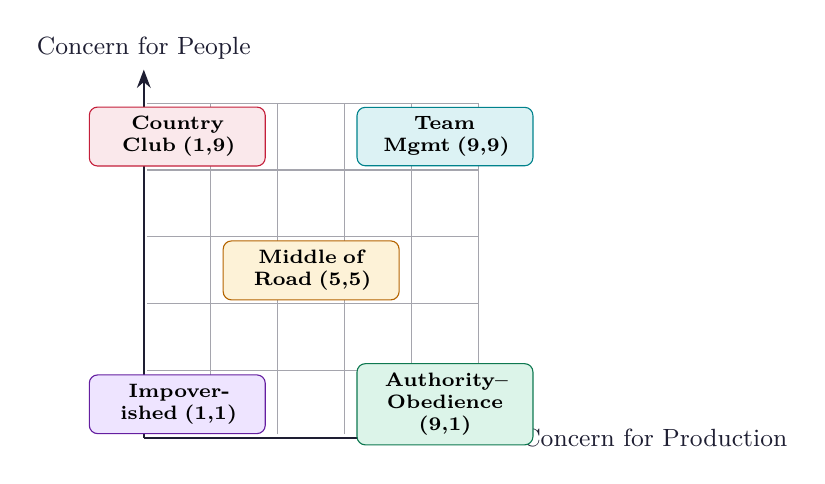
\begin{tikzpicture}[scale=0.85]
  \draw[-Stealth, thick, color=mydark] (0,0) -- (5.5,0) node[right, font=\small] {Concern for Production};
  \draw[-Stealth, thick, color=mydark] (0,0) -- (0,5.5) node[above, font=\small] {Concern for People};

  \foreach \x in {1,2,3,4,5} \draw[color=mydark!40, thin] (\x,0.05)--(\x,5);
  \foreach \y in {1,2,3,4,5} \draw[color=mydark!40, thin] (0.05,\y)--(5,\y);

  \node[draw=myred, fill=hdrred, rounded corners=3pt, font=\scriptsize\bfseries,
    text width=2.0cm, align=center, minimum height=0.65cm] at (0.5,4.5) {Country Club (1,9)};
  \node[draw=myteal, fill=hdrteal, rounded corners=3pt, font=\scriptsize\bfseries,
    text width=2.0cm, align=center, minimum height=0.65cm] at (4.5,4.5) {Team Mgmt (9,9)};
  \node[draw=myamber, fill=hdramber, rounded corners=3pt, font=\scriptsize\bfseries,
    text width=2.0cm, align=center, minimum height=0.65cm] at (2.5,2.5) {Middle of Road (5,5)};
  \node[draw=mypurple, fill=hdrpurple, rounded corners=3pt, font=\scriptsize\bfseries,
    text width=2.0cm, align=center, minimum height=0.65cm] at (0.5,0.5) {Impoverished (1,1)};
  \node[draw=mygreen, fill=hdrgreen, rounded corners=3pt, font=\scriptsize\bfseries,
    text width=2.0cm, align=center, minimum height=0.65cm] at (4.5,0.5) {Authority--Obedience (9,1)};
\end{tikzpicture}
\end{tcolorbox}

\subsubsection{Situational/Contingency Theories}
Leadership effectiveness depends on the match between the leader's style and the situation:
\begin{itemize}[leftmargin=*, itemsep=2pt]
  \item \textbf{Fiedler's Contingency Model:} Leadership effectiveness depends on the match between the leader's style (task vs.\ relationship oriented) and situational favourableness (leader--member relations, task structure, position power).
  \item \textbf{Hersey--Blanchard Situational Leadership:} Leader adapts style (Telling $\to$ Selling $\to$ Participating $\to$ Delegating) based on follower \textit{readiness} (competence + commitment).
  \item \textbf{Path--Goal Theory (House):} Leader's job is to remove obstacles and provide guidance (directive, supportive, participative, achievement-oriented) to help followers reach their goals.
\end{itemize}

% ===============================================================================
\section{Decision Making}
% ===============================================================================

\begin{tcolorbox}[defbox, title={\textbf{Decision Making --- Definition}}]
\textbf{Decision Making} is the process of identifying and selecting a course of action to solve a specific problem or capitalise on an opportunity. It is the core of managerial activity and involves choosing among alternatives under conditions of certainty, risk, or uncertainty.
\end{tcolorbox}

\subsection{Concept and Nature of Decision Making}
\begin{itemize}[leftmargin=*, itemsep=3pt]
  \item \textbf{Pervasive:} Decision making occurs at all levels and in all functions of management.
  \item \textbf{Continuous:} Managers make decisions constantly throughout their working day.
  \item \textbf{Goal-Directed:} Every decision is aimed at solving a problem or achieving an objective.
  \item \textbf{Selection Among Alternatives:} Decision making implies the existence of two or more possible choices.
\end{itemize}

\subsection{Types of Decisions}
\par\noindent
\begin{tabularx}{\linewidth}{|B{3.2cm}|Y|Y|}
\hline
\rowcolor{hdrgray}
\multicolumn{1}{|>{\centering\arraybackslash}m{3.2cm}|}{\textbf{Type}} &
\multicolumn{1}{>{\centering\arraybackslash}Y|}{\textbf{Description}} &
\multicolumn{1}{>{\centering\arraybackslash}Y|}{\textbf{Example}} \\
\hline
Programmed (Structured) & Routine, repetitive decisions handled by standard procedures and rules. & Processing a standard purchase order. \\
\hline
Non-Programmed (Unstructured) & Novel, complex, non-routine decisions requiring judgment. & Entering a new international market. \\
\hline
Strategic & Long-term, top-level decisions affecting the entire organisation. & Mergers and acquisitions. \\
\hline
Tactical & Medium-term decisions by middle management to implement strategy. & Annual budget allocation. \\
\hline
Operational & Short-term, day-to-day decisions at the operational level. & Employee shift scheduling. \\
\hline
\end{tabularx}

\subsection{The Decision-Making Process}

\begin{tcolorbox}[tikzbox, title={Rational Decision-Making Process}]
\centering
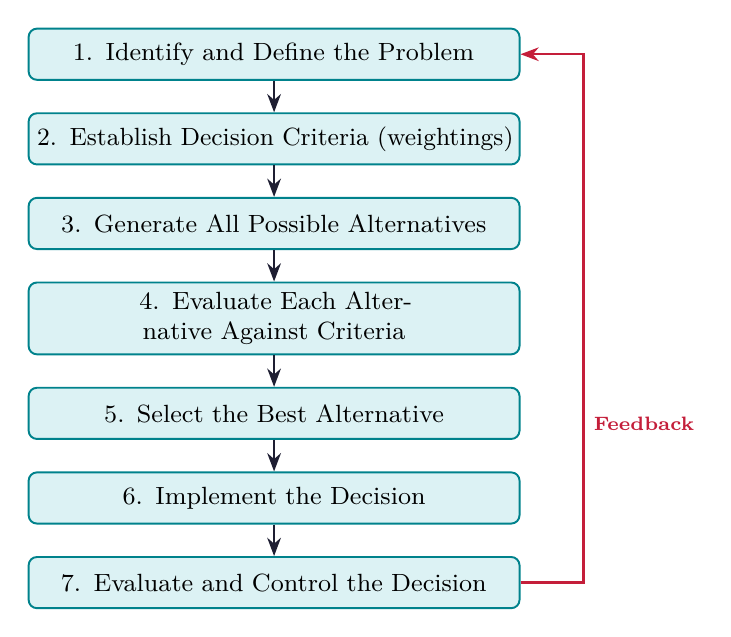
\begin{tikzpicture}[
  stepbox/.style={rectangle, draw=myteal, fill=hdrteal, text width=6.0cm,
    align=center, minimum height=0.65cm, font=\small, rounded corners=3pt, line width=0.7pt},
  arrow/.style={-Stealth, thick, color=mydark}
]
  \node[stepbox] (s1) {1. Identify and Define the Problem};
  \node[stepbox, below=0.4cm of s1] (s2) {2. Establish Decision Criteria (weightings)};
  \node[stepbox, below=0.4cm of s2] (s3) {3. Generate All Possible Alternatives};
  \node[stepbox, below=0.4cm of s3] (s4) {4. Evaluate Each Alternative Against Criteria};
  \node[stepbox, below=0.4cm of s4] (s5) {5. Select the Best Alternative};
  \node[stepbox, below=0.4cm of s5] (s6) {6. Implement the Decision};
  \node[stepbox, below=0.4cm of s6] (s7) {7. Evaluate and Control the Decision};

  \draw[arrow] (s1)--(s2); \draw[arrow] (s2)--(s3); \draw[arrow] (s3)--(s4);
  \draw[arrow] (s4)--(s5); \draw[arrow] (s5)--(s6); \draw[arrow] (s6)--(s7);
  \draw[redarrow] (s7.east) -- ++(0.8,0) |- (s1.east)
    node[pos=0.15, right, font=\scriptsize\bfseries\color{myred}] {Feedback};
\end{tikzpicture}
\end{tcolorbox}

\subsection{Decision-Making Tools and Techniques}

\begin{itemize}[leftmargin=*, itemsep=3pt]
  \item \textbf{Brainstorming:} Group technique for generating maximum creative alternatives without criticism.
  \item \textbf{Delphi Technique:} Structured consensus-building among experts through successive anonymous questionnaires.
  \item \textbf{Decision Tree:} A graphical tool showing a sequence of decisions and their possible outcomes, payoffs, and probabilities.
  \item \textbf{Pay-off Matrix:} A table showing payoffs for each decision under each state of nature; used under uncertainty.
  \item \textbf{Cost--Benefit Analysis (CBA):} Compares the total expected costs and benefits of alternatives; choose the alternative with the highest net benefit.
  \item \textbf{Linear Programming (LP):} Optimises an objective function (maximise profit, minimise cost) subject to linear constraints.
  \item \textbf{SWOT Analysis:} Evaluates Strengths, Weaknesses, Opportunities, and Threats to guide strategic decisions.
\end{itemize}

% ===============================================================================
\section{Economic, Financial and Quantitative Analysis}
% ===============================================================================

\subsection{Production and Markets}

\begin{tcolorbox}[defbox, title={\textbf{Production and Market Structures}}]
\textbf{Production} is the process of transforming inputs (labour, capital, raw materials) into outputs (goods and services). Market structure defines the competitive environment in which firms operate.
\end{tcolorbox}

\par\noindent
\begin{tabularx}{\linewidth}{|B{2.8cm}|Y|Y|Y|}
\hline
\rowcolor{hdrgray}
\multicolumn{1}{|>{\centering\arraybackslash}m{2.8cm}|}{\textbf{Structure}} &
\multicolumn{1}{>{\centering\arraybackslash}Y|}{\textbf{Sellers}} &
\multicolumn{1}{>{\centering\arraybackslash}Y|}{\textbf{Price Control}} &
\multicolumn{1}{>{\centering\arraybackslash}Y|}{\textbf{Example}} \\
\hline
Perfect Competition & Many & None (price takers) & Agricultural markets. \\
\hline
Monopolistic Competition & Many & Some (product differentiation) & Restaurants, clothing. \\
\hline
Oligopoly & Few & Significant & Telecom, automobile. \\
\hline
Monopoly & One & Full (price maker) & Utility companies. \\
\hline
\end{tabularx}

\subsection{National Income Accounting}

\begin{tcolorbox}[formulabox, title={\textbf{National Income Concepts}}]
\renewcommand{\arraystretch}{1.3}
\begin{tabularx}{\linewidth}{B{4.5cm} X}
GDP (Expenditure) & $\text{GDP} = C + I + G + (X - M)$ \\[4pt]
NNP at Market Price & $\text{NNP}_{MP} = \text{GNP}_{MP} - \text{Depreciation}$ \\[4pt]
National Income (NI) & $\text{NI} = \text{NNP}_{MP} - \text{Indirect Taxes} + \text{Subsidies}$ \\[4pt]
Personal Income & $\text{PI} = \text{NI} - \text{Retained Earnings} - \text{Corp.\ Taxes} + \text{Transfer Payments}$ \\[4pt]
Disposable Income & $\text{DI} = \text{PI} - \text{Personal Taxes}$
\end{tabularx}
\par\vspace{4pt}
Where: $C$ = Consumption, $I$ = Investment, $G$ = Government spending, $X - M$ = Net exports.
\end{tcolorbox}

\subsection{Financial Statement Analysis}

\begin{tcolorbox}[defbox, title={\textbf{Financial Statements}}]
\textbf{Balance Sheet:} Snapshot of financial position at a point in time (Assets = Liabilities + Equity).
\par\vspace{3pt}
\textbf{Income Statement (P\&L):} Shows revenues, expenses, and profit/loss over a period.
\par\vspace{3pt}
\textbf{Cash Flow Statement:} Tracks actual cash inflows and outflows from operations, investing, and financing activities.
\end{tcolorbox}

\textbf{Key Financial Ratios:}\par\noindent
\begin{tabularx}{\linewidth}{|B{3.2cm}|Y|Y|}
\hline
\rowcolor{myteal}
\multicolumn{1}{|>{\centering\arraybackslash\color{white}}m{3.2cm}|}{\textbf{Category}} &
\multicolumn{1}{>{\centering\arraybackslash\color{white}}Y|}{\textbf{Ratio}} &
\multicolumn{1}{>{\centering\arraybackslash\color{white}}Y|}{\textbf{Formula}} \\
\hline
Liquidity & Current Ratio & Current Assets / Current Liabilities \\
\hline
Liquidity & Quick Ratio & (Current Assets $-$ Inventory) / Current Liabilities \\
\hline
Profitability & Net Profit Margin & Net Profit / Net Sales $\times$ 100 \\
\hline
Profitability & Return on Equity (ROE) & Net Profit / Shareholders' Equity $\times$ 100 \\
\hline
Leverage & Debt-to-Equity & Total Debt / Shareholders' Equity \\
\hline
Activity & Inventory Turnover & Cost of Goods Sold / Average Inventory \\
\hline
\end{tabularx}

\subsection{Quantitative Methods --- Statistical Inference}

\begin{tcolorbox}[defbox, title={\textbf{Statistical Inference}}]
\textbf{Statistical Inference} is the process of drawing conclusions about population parameters based on data from a sample. Key concepts: hypothesis testing, confidence intervals, and significance levels.
\end{tcolorbox}

\begin{tcolorbox}[formulabox, title={\textbf{Hypothesis Testing --- Z-test for Population Mean}}]
\renewcommand{\arraystretch}{1.3}
\begin{tabularx}{\linewidth}{B{4.0cm} X}
Test Statistic & $\displaystyle z = \frac{\bar{x} - \mu_0}{\sigma / \sqrt{n}}$ \\[8pt]
Standard Error & $\displaystyle SE = \frac{\sigma}{\sqrt{n}}$ \\[8pt]
Confidence Interval & $\displaystyle \mu \in \left(\bar{x} - z_{\alpha/2} \cdot SE,\;\; \bar{x} + z_{\alpha/2} \cdot SE\right)$
\end{tabularx}
\par\vspace{4pt}
Reject $H_0$ if $|z| > z_{\alpha/2}$ (two-tailed test). Common: $z_{0.025} = 1.96$ for 95\% confidence.
\end{tcolorbox}

\subsection{Forecasting}

\begin{tcolorbox}[defbox, title={\textbf{Forecasting}}]
\textbf{Forecasting} is the process of using historical data, trends, and judgments to predict future values (demand, sales, costs). It reduces uncertainty in planning and decision-making.
\end{tcolorbox}

\textbf{Common forecasting methods:}
\begin{itemize}[leftmargin=*, itemsep=2pt]
  \item \textbf{Moving Average:} Average of the most recent $n$ data points; smooths out fluctuations.
  \item \textbf{Exponential Smoothing:} Weighted moving average where more recent data receives greater weight.
  \item \textbf{Trend Projection:} Fits a least-squares regression line to historical data and projects it forward.
  \item \textbf{Qualitative methods:} Delphi, market surveys, jury of executive opinion --- used when historical data is absent.
\end{itemize}

\begin{tcolorbox}[formulabox, title={\textbf{Simple Linear Regression (Trend Line)}}]
\renewcommand{\arraystretch}{1.3}
\begin{tabularx}{\linewidth}{B{4.0cm} X}
Regression Line & $\hat{y} = a + bx$ \\[4pt]
Slope & $\displaystyle b = \frac{n\sum xy - \sum x \sum y}{n \sum x^2 - \left(\sum x\right)^2}$ \\[8pt]
Intercept & $\displaystyle a = \frac{\sum y - b\sum x}{n}$ \\[6pt]
Correlation Coefficient & $\displaystyle r = \frac{n\sum xy - \sum x \sum y}{\sqrt{[n\sum x^2 - (\sum x)^2][n\sum y^2 - (\sum y)^2]}}$
\end{tabularx}
\par\vspace{4pt}
$|r| = 1$: perfect correlation; $r = 0$: no linear correlation. $r^2$ (coefficient of determination) measures the proportion of variance explained.
\end{tcolorbox}

\subsection{Statistical Quality Control (SQC)}

\begin{tcolorbox}[defbox, title={\textbf{Statistical Quality Control (SQC)}}]
\textbf{SQC} is the application of statistical methods to monitor and control a production process so that the process operates at its full potential and produces conforming products.
\end{tcolorbox}

\textbf{Key tools of SQC:}
\begin{itemize}[leftmargin=*, itemsep=3pt]
  \item \textbf{Control Charts:} Monitor process variation over time. Central Line (CL), Upper Control Limit (UCL), and Lower Control Limit (LCL) are plotted. Common types: $\bar{X}$-chart (mean), R-chart (range), p-chart (proportion defective).
  \item \textbf{Acceptance Sampling:} Inspecting a random sample from a batch; accept or reject the entire batch based on the sample result.
  \item \textbf{Process Capability Index ($C_p$, $C_{pk}$):} Measures how well a process meets specifications.
\end{itemize}

\begin{tcolorbox}[formulabox, title={\textbf{Control Chart Limits for \texorpdfstring{$\bar{X}$}{X-bar} Chart}}]
\renewcommand{\arraystretch}{1.3}
\begin{tabularx}{\linewidth}{B{3.5cm} X}
Centre Line (CL) & $\bar{\bar{X}}$ (grand mean of all subgroup means) \\[4pt]
Upper Control Limit & $\text{UCL} = \bar{\bar{X}} + A_2 \bar{R}$ \\[4pt]
Lower Control Limit & $\text{LCL} = \bar{\bar{X}} - A_2 \bar{R}$
\end{tabularx}
\par\vspace{4pt}
$A_2$ = tabulated constant based on subgroup size $n$; $\bar{R}$ = average range.
A point outside UCL or LCL signals an \textbf{out-of-control} (assignable cause) condition.
\end{tcolorbox}

% ===============================================================================
% MANDATORY QUICK REVISION PAGE
% ===============================================================================
\newpage
\begin{center}
  {\large\bfseries\color{myred} Quick Revision --- Module 3}\\[3pt]
  {\small\color{mydark} Leadership, Decision Making \& Quantitative Analysis $|$ HS-HU701}
\end{center}
\noindent{\color{myred}\rule{\linewidth}{1.2pt}}
\vspace{4pt}

\begin{tcolorbox}[formulabox, title={\textbf{Key Formulas at a Glance}}]
\renewcommand{\arraystretch}{1.3}
\begin{tabularx}{\linewidth}{B{4.2cm} X}
GDP (Expenditure) & $C + I + G + (X - M)$ \\[3pt]
National Income & $\text{GNP}_{MP} - \text{Depreciation} - \text{Indirect Taxes} + \text{Subsidies}$ \\[3pt]
Z-test Statistic & $z = (\bar{x} - \mu_0) / (\sigma / \sqrt{n})$ \\[3pt]
Regression Slope & $b = (n\sum xy - \sum x \sum y) / (n\sum x^2 - (\sum x)^2)$ \\[3pt]
X-bar UCL / LCL & $\bar{\bar{X}} \pm A_2 \bar{R}$ \\[3pt]
Current Ratio & Current Assets / Current Liabilities \\[3pt]
Net Profit Margin & Net Profit / Net Sales $\times 100$ \\
\end{tabularx}
\end{tcolorbox}

\begin{tcolorbox}[defbox, title={\textbf{One-Line Definitions}}]
\begin{itemize}[leftmargin=*, itemsep=2pt, topsep=0pt]
  \item \textbf{Leadership:} Ability to influence and guide others toward achieving goals.
  \item \textbf{Autocratic Leadership:} Leader makes all decisions unilaterally with full authority.
  \item \textbf{Transformational Leadership:} Inspires change through vision, charisma, and motivation.
  \item \textbf{Decision Making:} Process of selecting a course of action from available alternatives.
  \item \textbf{Programmed Decision:} Routine decision resolved by standard procedures.
  \item \textbf{Non-Programmed Decision:} Novel, complex decision requiring managerial judgment.
  \item \textbf{GDP:} Total monetary value of all goods and services produced within a country in a year.
  \item \textbf{SQC:} Use of statistical methods to monitor and control production quality.
  \item \textbf{Control Chart:} Graphical tool to detect process variation over time using UCL and LCL.
  \item \textbf{Regression Analysis:} Statistical method to model the relationship between variables.
  \item \textbf{Forecasting:} Using historical data and trends to predict future values.
\end{itemize}
\end{tcolorbox}

\begin{tcolorbox}[exambox, title={\textbf{Frequently Asked / Viva Questions}}]
\begin{enumerate}[topsep=0pt, label=\textbf{Q\arabic*.}, itemsep=5pt]
  \item \Q{What is leadership? How does a leader differ from a manager?}
    Leadership is the ability to influence others toward goals. A manager has formal authority (appointed), while a leader may be informal. Managers administer; leaders innovate. Leaders inspire; managers control.
  \item \Q{Name and explain the three basic leadership styles.}
    Autocratic (leader decides alone), Democratic (team participates in decisions), Laissez-Faire (leader delegates fully with minimal intervention).
  \item \Q{What is the Blake--Mouton Managerial Grid? What is the ideal position?}
    A grid plotting concern for production (x-axis) vs.\ concern for people (y-axis), each on a 1--9 scale. The ideal position is (9,9) Team Management --- high concern for both people and production.
  \item \Q{What is Hersey--Blanchard Situational Leadership theory?}
    Leaders adapt their style (Telling $\to$ Selling $\to$ Participating $\to$ Delegating) based on the follower's readiness level (combination of competence and commitment).
  \item \Q{Distinguish between programmed and non-programmed decisions.}
    Programmed decisions are routine and repetitive, handled by standard rules (e.g., stock reorder). Non-programmed decisions are novel and complex, requiring judgment (e.g., entering a new market).
  \item \Q{What is the Decision Tree technique?}
    A graphical representation of a decision problem showing decision nodes (squares), chance nodes (circles), possible outcomes, and associated probabilities and payoffs, enabling rational selection of the best path.
  \item \Q{What is GDP? Write its expenditure-side formula.}
    GDP (Gross Domestic Product) is the total monetary value of all final goods and services produced within a country in a year. Expenditure formula: $\text{GDP} = C + I + G + (X - M)$.
  \item \Q{What is Statistical Quality Control (SQC)? Name its key tools.}
    SQC is the use of statistical methods to monitor and control production processes. Key tools: Control Charts ($\bar{X}$-chart, R-chart, p-chart), Acceptance Sampling, and Process Capability Indices.
  \item \Q{What do UCL and LCL represent in a control chart?}
    UCL (Upper Control Limit) and LCL (Lower Control Limit) are the boundaries of natural process variation (set at $\pm 3\sigma$). A plotted point outside these limits indicates an out-of-control (assignable cause) condition.
  \item \Q{State the formula for simple linear regression.}
    $\hat{y} = a + bx$, where $b$ is the slope and $a$ is the intercept. The slope is $b = (n\sum xy - \sum x \sum y) / (n\sum x^2 - (\sum x)^2)$.
  \item \Q{What is the purpose of financial ratio analysis?}
    It allows comparison of a firm's performance against its own historical data, competitors, or industry benchmarks. Key categories: liquidity (current ratio), profitability (ROE), leverage (debt-to-equity), and activity (inventory turnover).
  \item \Q{What is the difference between Transformational and Transactional leadership?}
    Transformational leaders inspire change through vision and motivation (long-term focus). Transactional leaders use reward--punishment to maintain performance within existing norms (short-term, routine focus).
\end{enumerate}
\end{tcolorbox}

\begin{tcolorbox}[tikzbox, title={Types of Decisions --- Comparison Table}]
\centering
\renewcommand{\arraystretch}{1.4}
\begin{tabularx}{\linewidth}{|B{3.0cm}|Y|Y|}
\hline
\rowcolor{hdrgray}
\multicolumn{1}{|>{\centering\arraybackslash}m{3.0cm}|}{\textbf{Aspect}} &
\multicolumn{1}{>{\centering\arraybackslash}Y|}{\textbf{Programmed Decision}} &
\multicolumn{1}{>{\centering\arraybackslash}Y|}{\textbf{Non-Programmed Decision}} \\
\hline
Nature & Routine, repetitive & Novel, unique \\
\hline
Level & Lower/Middle management & Top management \\
\hline
Time & Short-term & Long-term \\
\hline
Basis & Standard rules, procedures & Judgment, creativity \\
\hline
Risk & Low & High \\
\hline
Example & Payroll processing & Product launch strategy \\
\hline
\end{tabularx}
\end{tcolorbox}


% -- Module 4 -----------------------------------------------------------------
\modulestart{4}{Customer Management}

\section{Customer Management}
% ===============================================================================

\begin{tcolorbox}[defbox, title={\textbf{Customer Management --- Overview}}]
\textbf{Customer Management} encompasses all strategies and activities through which an organisation attracts, retains, and grows its customer base. It includes market planning, research, the marketing mix, advertising, and brand management --- all directed toward satisfying customer needs profitably.
\end{tcolorbox}

\subsection{Market Planning and Research}

\begin{tcolorbox}[defbox, title={\textbf{Market Planning and Marketing Research}}]
\textbf{Market Planning} is the process of setting marketing objectives and devising strategies and tactics to achieve them. It involves analysing the market environment, identifying target segments, and allocating resources.
\par\vspace{3pt}
\textbf{Marketing Research} is the systematic gathering, recording, and analysis of data about problems relating to the marketing of goods and services. It bridges the gap between the organisation and its customers.
\end{tcolorbox}

\textbf{Steps in the Marketing Research Process:}
\begin{enumerate}[label=\textbf{\arabic*.}, leftmargin=*, itemsep=3pt, topsep=2pt]
  \item \textbf{Define the Problem and Research Objectives:} Clearly state what information is needed.
  \item \textbf{Develop the Research Plan:} Choose data sources (primary/secondary), research methods (survey, observation, experiment), and sampling plan.
  \item \textbf{Collect Information:} Gather primary data (questionnaires, interviews, focus groups) or secondary data (reports, databases).
  \item \textbf{Analyse the Information:} Tabulate, cross-tabulate, and apply statistical techniques.
  \item \textbf{Present the Findings:} Report actionable conclusions to management.
  \item \textbf{Make the Decision:} Use findings to guide marketing strategy.
\end{enumerate}

\subsection{The Marketing Mix --- 4Ps}

\begin{tcolorbox}[defbox, title={\textbf{Marketing Mix (4Ps)}}]
The \textbf{Marketing Mix} is the set of controllable, tactical marketing tools that the firm blends to produce the response it wants in the target market. The four Ps are: \textbf{Product, Price, Place (Distribution), and Promotion}.
\end{tcolorbox}

\begin{tcolorbox}[tikzbox, title={The 4Ps of the Marketing Mix}]
\centering
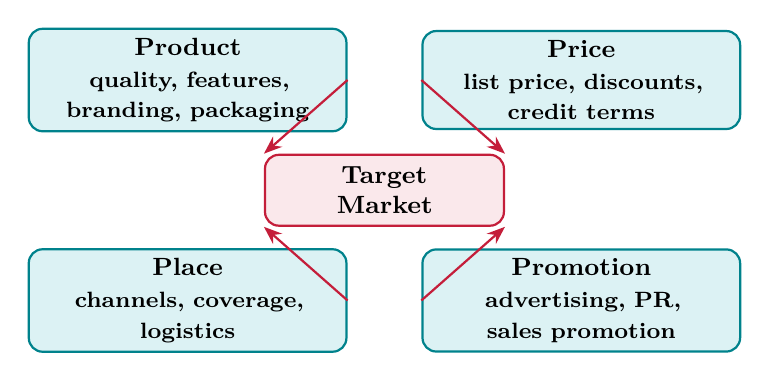
\begin{tikzpicture}[
  pbox/.style={rectangle, draw=myteal, fill=hdrteal, text width=3.8cm,
    align=center, minimum height=1.2cm, font=\small\bfseries,
    rounded corners=5pt, line width=0.8pt},
  tbox/.style={rectangle, draw=myred, fill=hdrred, text width=2.8cm,
    align=center, minimum height=0.9cm, font=\small\bfseries,
    rounded corners=5pt, line width=0.8pt}
]
  % 2x2 grid of P-boxes
  \node[pbox] (prod)  at (-2.5,  1.4) {Product\\[2pt]{\footnotesize quality, features,\\branding, packaging}};
  \node[pbox] (price) at ( 2.5,  1.4) {Price\\[2pt]{\footnotesize list price, discounts,\\credit terms}};
  \node[pbox] (place) at (-2.5, -1.4) {Place\\[2pt]{\footnotesize channels, coverage,\\logistics}};
  \node[pbox] (promo) at ( 2.5, -1.4) {Promotion\\[2pt]{\footnotesize advertising, PR,\\sales promotion}};

  % Central target node
  \node[tbox] (tm) at (0, 0) {\textbf{Target\\Market}};

  % Arrows from each P to target
  \draw[redarrow] (prod.east)  -- (tm.north west);
  \draw[redarrow] (price.west) -- (tm.north east);
  \draw[redarrow] (place.east) -- (tm.south west);
  \draw[redarrow] (promo.west) -- (tm.south east);
\end{tikzpicture}
\end{tcolorbox}

\par\noindent
\begin{tabularx}{\linewidth}{|B{2.2cm}|Y|Y|}
\hline
\rowcolor{myteal}
\multicolumn{1}{|>{\centering\arraybackslash\color{white}}m{2.2cm}|}{\textbf{Element}} &
\multicolumn{1}{>{\centering\arraybackslash\color{white}}Y|}{\textbf{Key Decisions}} &
\multicolumn{1}{>{\centering\arraybackslash\color{white}}Y|}{\textbf{Examples}} \\
\hline
Product & Design, quality, features, variants, packaging, after-sales service. & iPhone with multiple storage options. \\
\hline
Price & Pricing strategy (skimming, penetration, competitive), discounts, payment terms. & Introductory low price for market entry. \\
\hline
Place & Distribution channels, intermediaries, logistics, coverage (intensive, selective, exclusive). & Direct online sale vs.\ retail chain. \\
\hline
Promotion & Advertising, personal selling, public relations, sales promotions, digital marketing. & TV ad campaign + social media promotion. \\
\hline
\end{tabularx}

\subsection{Advertising and Brand Management}

\begin{tcolorbox}[defbox, title={\textbf{Advertising and Brand Management}}]
\textbf{Advertising} is any paid form of non-personal presentation and promotion of ideas, goods, or services by an identified sponsor through mass media (TV, radio, print, digital).
\par\vspace{3pt}
\textbf{Brand} is a name, term, sign, symbol, or design (or a combination) intended to identify the goods or services of one seller and to differentiate them from competitors.
\par\vspace{3pt}
\textbf{Brand Equity} is the added value a brand name gives to a product beyond its functional benefits.
\end{tcolorbox}

\textbf{Objectives of Advertising (AIDA Model):}
\begin{enumerate}[label=\textbf{\arabic*.}, leftmargin=*, itemsep=2pt, topsep=2pt]
  \item \textbf{Awareness:} Make the target audience aware of the product/brand.
  \item \textbf{Interest:} Generate interest by highlighting features and benefits.
  \item \textbf{Desire:} Create a desire/preference for the brand over competitors.
  \item \textbf{Action:} Motivate the consumer to purchase.
\end{enumerate}

\textbf{Brand building strategies:}
\begin{itemize}[leftmargin=*, itemsep=2pt]
  \item Consistent quality and customer experience across all touchpoints.
  \item Emotional brand associations and storytelling.
  \item Celebrity endorsements and influencer marketing.
  \item Corporate Social Responsibility (CSR) initiatives that enhance brand image.
\end{itemize}

% ===============================================================================
\section{Operations and Technology Management}
% ===============================================================================

\begin{tcolorbox}[defbox, title={\textbf{Operations Management --- Definition}}]
\textbf{Operations Management (OM)} is the administration of business practices aimed at creating the highest level of efficiency possible within an organisation. It is concerned with converting materials and labour into goods and services as efficiently as possible.
\end{tcolorbox}

\subsection{Production and Operations Management}

\textbf{Types of production systems:}
\par\noindent
\begin{tabularx}{\linewidth}{|B{3.0cm}|Y|Y|}
\hline
\rowcolor{hdrgray}
\multicolumn{1}{|>{\centering\arraybackslash}m{3.0cm}|}{\textbf{Type}} &
\multicolumn{1}{>{\centering\arraybackslash}Y|}{\textbf{Description}} &
\multicolumn{1}{>{\centering\arraybackslash}Y|}{\textbf{Example}} \\
\hline
Job/Project Production & One-off, custom products made individually. & Ship building, construction. \\
\hline
Batch Production & Groups of identical items produced together in stages. & Bakeries, pharmaceuticals. \\
\hline
Mass/Flow Production & Continuous, standardised production of large volumes on assembly lines. & Car assembly, electronics. \\
\hline
Continuous Process & 24/7 uninterrupted flow production. & Oil refinery, chemical plant. \\
\hline
\end{tabularx}

\textbf{Key decisions in Production/Operations Management:}
\begin{itemize}[leftmargin=*, itemsep=2pt]
  \item \textbf{Capacity planning:} Determining production capacity needed to meet demand.
  \item \textbf{Facility layout:} Arrangement of machines, workstations, and storage (process layout, product layout, fixed-position layout).
  \item \textbf{Aggregate planning:} Medium-term production scheduling to match supply with forecasted demand.
  \item \textbf{Inventory management:} Deciding optimal stock levels to balance holding costs vs.\ shortage costs.
\end{itemize}

\begin{tcolorbox}[formulabox, title={\textbf{Economic Order Quantity (EOQ)}}]
The EOQ model minimises total inventory cost (holding + ordering):
\begin{equation}
  Q^* = \sqrt{\frac{2DS}{H}}
\end{equation}
Where:
\begin{itemize}[leftmargin=1.5em, itemsep=1pt, topsep=2pt]
  \item[] $Q^*$ = Optimal order quantity (units)
  \item[] $D$ = Annual demand (units/year)
  \item[] $S$ = Ordering cost per order (\$)
  \item[] $H$ = Annual holding/carrying cost per unit
\end{itemize}
\par\vspace{4pt}
Total Annual Cost: $\displaystyle TC = \frac{D}{Q}S + \frac{Q}{2}H$
\end{tcolorbox}

\subsection{Logistics and Supply Chain Management}

\begin{tcolorbox}[defbox, title={\textbf{Supply Chain Management (SCM)}}]
\textbf{Supply Chain Management} is the management of the flow of goods, services, information, and finances from raw material suppliers through manufacturers and distributors to the final end-user. The goal is to maximise customer value while minimising total system cost.
\end{tcolorbox}

\begin{tcolorbox}[tikzbox, title={Basic Supply Chain Flow}]
\centering
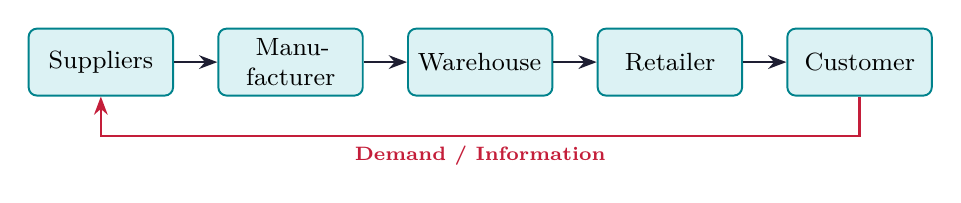
\begin{tikzpicture}[node distance=0.3cm and 0.5cm,
  sblock/.style={rectangle, draw=myteal, fill=hdrteal, text width=1.6cm,
    align=center, minimum height=0.85cm, font=\small, rounded corners=3pt, line width=0.7pt}]
  \node[sblock] (sup) {Suppliers};
  \node[sblock, right=0.55cm of sup] (mfg) {Manufacturer};
  \node[sblock, right=0.55cm of mfg] (wh)  {Warehouse};
  \node[sblock, right=0.55cm of wh]  (ret) {Retailer};
  \node[sblock, right=0.55cm of ret] (cust){Customer};

  \draw[arrow] (sup)--(mfg);
  \draw[arrow] (mfg)--(wh);
  \draw[arrow] (wh)--(ret);
  \draw[arrow] (ret)--(cust);
  \draw[redarrow] (cust.south) -- ++(0,-0.5) -| (sup.south)
    node[pos=0.25, below, font=\scriptsize\bfseries\color{myred}] {Demand / Information};
\end{tikzpicture}
\end{tcolorbox}

\textbf{Key logistics activities:}
\begin{itemize}[leftmargin=*, itemsep=2pt]
  \item Transportation (road, rail, air, sea selection).
  \item Warehousing and inventory storage.
  \item Order processing and fulfilment.
  \item Demand forecasting and supply planning.
  \item Reverse logistics (returns, recycling).
\end{itemize}

\subsection{Total Quality Management (TQM)}

\begin{tcolorbox}[defbox, title={\textbf{Total Quality Management (TQM)}}]
\textbf{TQM} is a management approach centred on quality, based on the participation of all members of an organisation, aimed at long-term success through customer satisfaction and benefits to all members of the organisation and society.
\par\vspace{3pt}
\textbf{Core principle:} Quality is everyone's responsibility, not just the quality control department.
\end{tcolorbox}

\textbf{Key principles of TQM:}
\begin{itemize}[leftmargin=*, itemsep=2pt]
  \item \textbf{Customer Focus:} Understanding and exceeding customer expectations.
  \item \textbf{Continuous Improvement (Kaizen):} Ongoing, incremental improvements in all processes.
  \item \textbf{Employee Involvement:} All employees contribute to quality improvement.
  \item \textbf{Process Approach:} Focus on improving processes to improve outputs.
  \item \textbf{Fact-Based Decision Making:} Use of data and statistical tools.
  \item \textbf{Supplier Relationships:} Mutually beneficial relationships with suppliers.
\end{itemize}

\subsection{Kaizen and Six Sigma}

\begin{tcolorbox}[defbox, title={\textbf{Kaizen and Six Sigma}}]
\textbf{Kaizen} (Japanese: ``change for better'') is a philosophy of continuous, incremental improvement involving everyone in the organisation --- from top management to shop floor workers. It focuses on eliminating waste (Muda) in all forms.
\par\vspace{3pt}
\textbf{Six Sigma} is a data-driven methodology for eliminating defects in any process. The goal is to reduce process variation to achieve no more than \textbf{3.4 defects per million opportunities (DPMO)}.
\end{tcolorbox}

\textbf{Kaizen vs.\ Six Sigma:}
\par\noindent
\begin{tabularx}{\linewidth}{|B{3.0cm}|Y|Y|}
\hline
\rowcolor{hdrgray}
\multicolumn{1}{|>{\centering\arraybackslash}m{3.0cm}|}{\textbf{Aspect}} &
\multicolumn{1}{>{\centering\arraybackslash}Y|}{\textbf{Kaizen}} &
\multicolumn{1}{>{\centering\arraybackslash}Y|}{\textbf{Six Sigma}} \\
\hline
Origin & Japan (Toyota Production System) & Motorola (1986) \\
\hline
Approach & Incremental, continuous improvement. & Breakthrough improvement; eliminate root causes of defects. \\
\hline
Scope & Entire organisation; all processes. & Specific critical processes and projects. \\
\hline
Tools & 5S, PDCA, Value Stream Mapping. & DMAIC, statistical tools (SPC, DOE). \\
\hline
Involvement & All employees (bottom-up). & Trained specialists (Black Belts, Green Belts). \\
\hline
Goal & Reduce waste; improve efficiency. & Reduce variation; achieve near-zero defects. \\
\hline
\end{tabularx}

\textbf{The DMAIC Cycle (Six Sigma):}
\begin{enumerate}[label=\textbf{\arabic*.}, leftmargin=*, itemsep=2pt, topsep=2pt]
  \item \textbf{Define:} Define the problem, project scope, customer requirements (CTQs), and project goals.
  \item \textbf{Measure:} Collect baseline data; quantify the current process performance.
  \item \textbf{Analyse:} Identify root causes of defects using statistical tools (Fishbone diagram, Pareto chart, regression).
  \item \textbf{Improve:} Develop, test, and implement solutions to eliminate root causes.
  \item \textbf{Control:} Monitor the improved process to sustain gains using control charts and SOPs.
\end{enumerate}

\textbf{The PDCA Cycle (Kaizen / TQM):}
\begin{enumerate}[label=\textbf{\arabic*.}, leftmargin=*, itemsep=2pt, topsep=2pt]
  \item \textbf{Plan:} Identify a problem; analyse causes; plan improvement.
  \item \textbf{Do:} Implement the planned change on a small scale.
  \item \textbf{Check:} Measure and evaluate results against the plan.
  \item \textbf{Act:} Standardise the improvement if successful; repeat the cycle.
\end{enumerate}

\subsection{Management Information Systems (MIS)}

\begin{tcolorbox}[defbox, title={\textbf{Management Information System (MIS)}}]
\textbf{MIS} is an integrated, user-machine system that provides information to support operations, management, and decision-making functions in an organisation. It collects data from internal and external sources, processes it, and presents it as structured reports and dashboards to managers.
\end{tcolorbox}

\textbf{Types of Information Systems:}
\par\noindent
\begin{tabularx}{\linewidth}{|B{3.2cm}|Y|Y|}
\hline
\rowcolor{myteal}
\multicolumn{1}{|>{\centering\arraybackslash\color{white}}m{3.2cm}|}{\textbf{System}} &
\multicolumn{1}{>{\centering\arraybackslash\color{white}}Y|}{\textbf{Level}} &
\multicolumn{1}{>{\centering\arraybackslash\color{white}}Y|}{\textbf{Purpose}} \\
\hline
TPS (Transaction Processing System) & Operational & Records daily routine transactions (sales, payroll). \\
\hline
MIS (Management Information System) & Middle management & Provides structured summary reports for routine decisions. \\
\hline
DSS (Decision Support System) & Middle/Top management & Supports semi-structured and unstructured decisions with models. \\
\hline
EIS/ESS (Executive Information System) & Top management & Strategic dashboards; external and internal data. \\
\hline
ERP (Enterprise Resource Planning) & All levels & Integrates all business functions (finance, HR, supply chain) in a single system. \\
\hline
\end{tabularx}

\textbf{Benefits of MIS:}
\begin{itemize}[leftmargin=*, itemsep=2pt]
  \item Facilitates faster and more accurate decision-making.
  \item Improves coordination and communication across departments.
  \item Provides real-time monitoring of business performance (KPIs).
  \item Reduces information redundancy and improves data integrity.
\end{itemize}

% ===============================================================================
% MANDATORY QUICK REVISION PAGE
% ===============================================================================
\newpage
\begin{center}
  {\large\bfseries\color{myred} Quick Revision --- Module 4}\\[3pt]
  {\small\color{mydark} Customer Management, Operations, TQM, Kaizen, Six Sigma \& MIS $|$ HS-HU701}
\end{center}
\noindent{\color{myred}\rule{\linewidth}{1.2pt}}
\vspace{4pt}

\begin{tcolorbox}[formulabox, title={\textbf{Key Formulas and Frameworks at a Glance}}]
\renewcommand{\arraystretch}{1.3}
\begin{tabularx}{\linewidth}{B{4.2cm} X}
EOQ & $Q^* = \sqrt{2DS/H}$ \\[4pt]
Total Inventory Cost & $TC = (D/Q)S + (Q/2)H$ \\[4pt]
4Ps of Marketing & Product, Price, Place, Promotion \\[3pt]
AIDA Model & Awareness $\to$ Interest $\to$ Desire $\to$ Action \\[3pt]
DMAIC (Six Sigma) & Define $\to$ Measure $\to$ Analyse $\to$ Improve $\to$ Control \\[3pt]
PDCA (Kaizen/TQM) & Plan $\to$ Do $\to$ Check $\to$ Act \\[3pt]
Six Sigma Target & $\leq$ 3.4 Defects Per Million Opportunities (DPMO) \\
\end{tabularx}
\end{tcolorbox}

\begin{tcolorbox}[defbox, title={\textbf{One-Line Definitions}}]
\begin{itemize}[leftmargin=*, itemsep=2pt, topsep=0pt]
  \item \textbf{Marketing Mix (4Ps):} Controllable tools (Product, Price, Place, Promotion) blended to target a market.
  \item \textbf{Brand Equity:} Extra value a brand name adds to a product beyond its functional benefits.
  \item \textbf{Operations Management:} Converting inputs (materials, labour) into goods/services as efficiently as possible.
  \item \textbf{EOQ:} Order quantity that minimises the sum of annual ordering cost and holding cost.
  \item \textbf{Supply Chain Management:} Managing the flow of goods and information from supplier to end customer.
  \item \textbf{TQM:} Organisation-wide approach to embedding quality in all processes to achieve customer satisfaction.
  \item \textbf{Kaizen:} Continuous, incremental improvement involving all employees to eliminate waste.
  \item \textbf{Six Sigma:} Data-driven methodology targeting $\leq$ 3.4 DPMO through root cause elimination.
  \item \textbf{DMAIC:} Six Sigma improvement cycle: Define, Measure, Analyse, Improve, Control.
  \item \textbf{MIS:} Integrated system that provides managers with information for decision-making.
  \item \textbf{ERP:} Software that integrates all core business processes into a single unified system.
\end{itemize}
\end{tcolorbox}

\begin{tcolorbox}[exambox, title={\textbf{Frequently Asked / Viva Questions}}]
\begin{enumerate}[topsep=0pt, label=\textbf{Q\arabic*.}, itemsep=5pt]
  \item \Q{What are the 4Ps of the Marketing Mix? Give one example for each.}
    Product (iPhone), Price (penetration pricing), Place (online store), Promotion (TV advertisement).
  \item \Q{What is the AIDA model in advertising?}
    AIDA stands for Awareness (make customers aware), Interest (highlight benefits), Desire (create preference), Action (prompt purchase). It describes the stages a consumer goes through from first exposure to buying.
  \item \Q{What is brand equity and why is it important?}
    Brand equity is the added value a brand name confers to a product. It is important because it enables premium pricing, customer loyalty, and competitive advantage (e.g., Apple vs.\ a generic smartphone).
  \item \Q{Define Supply Chain Management. Draw a simple supply chain.}
    SCM manages the flow of goods, services, and information from raw material suppliers to the final customer. Flow: Suppliers $\to$ Manufacturer $\to$ Warehouse $\to$ Retailer $\to$ Customer (with information flowing back).
  \item \Q{State the EOQ formula and define each variable.}
    $Q^* = \sqrt{2DS/H}$. $D$ = annual demand, $S$ = cost per order, $H$ = annual holding cost per unit. It gives the order quantity that minimises total annual inventory cost.
  \item \Q{What is TQM? What are its core principles?}
    TQM is an organisation-wide philosophy to embed quality in all processes for long-term customer satisfaction. Core principles: customer focus, continuous improvement, employee involvement, process approach, data-based decisions, and supplier relationships.
  \item \Q{What is Kaizen? How does it differ from Six Sigma?}
    Kaizen is continuous, incremental improvement through small daily changes involving all employees (bottom-up). Six Sigma is a project-based breakthrough methodology using statistical tools to reduce defects to 3.4 DPMO (specialist-driven).
  \item \Q{Explain the DMAIC cycle used in Six Sigma.}
    Define (problem and CTQs) $\to$ Measure (baseline performance) $\to$ Analyse (root causes) $\to$ Improve (implement solutions) $\to$ Control (sustain gains with control charts and SOPs).
  \item \Q{What is a Management Information System (MIS)?}
    MIS is an integrated system that collects, processes, and presents data as structured reports to support managerial decision-making at middle levels of the organisation.
  \item \Q{How does an ERP system differ from an MIS?}
    MIS provides reports for management decisions; ERP integrates all business functions (finance, HR, production, supply chain) across the entire organisation into one unified database and application.
  \item \Q{What is the PDCA cycle? Where is it used?}
    PDCA (Plan--Do--Check--Act) is a four-step iterative quality improvement cycle. Used in TQM and Kaizen to continuously improve processes, products, and services.
  \item \Q{What is the difference between intensive, selective, and exclusive distribution?}
    Intensive distribution places products in as many outlets as possible (e.g., soft drinks). Selective distribution uses a limited number of chosen outlets (e.g., electronics). Exclusive distribution uses a single outlet per region (e.g., luxury cars, high-end watches).
\end{enumerate}
\end{tcolorbox}

\begin{tcolorbox}[tikzbox, title={TQM vs.\ Kaizen vs.\ Six Sigma --- Quick Reference}]
\centering
\renewcommand{\arraystretch}{1.4}
\begin{tabularx}{\linewidth}{|B{2.5cm}|Y|Y|Y|}
\hline
\rowcolor{hdrgray}
\multicolumn{1}{|>{\centering\arraybackslash}m{2.5cm}|}{\textbf{Aspect}} &
\multicolumn{1}{>{\centering\arraybackslash}Y|}{\textbf{TQM}} &
\multicolumn{1}{>{\centering\arraybackslash}Y|}{\textbf{Kaizen}} &
\multicolumn{1}{>{\centering\arraybackslash}Y|}{\textbf{Six Sigma}} \\
\hline
Focus & Overall quality culture & Continuous small improvements & Eliminate defect root causes \\
\hline
Approach & Cultural/philosophical & Incremental (bottom-up) & Statistical/project-based \\
\hline
Cycle & PDCA & PDCA & DMAIC \\
\hline
People & Everyone & Everyone & Black/Green Belts \\
\hline
Target & Customer satisfaction & Waste elimination & $\leq$ 3.4 DPMO \\
\hline
\end{tabularx}
\end{tcolorbox}


\end{document}
